% !TeX root=main.tex
% دستور زیر باید در اولین فصل شما باشد. آن را حذف نکنید!
\pagenumbering{arabic}

\chapter{مقدمه}
\thispagestyle{empty}
\section{مقدمه}
حروف‌چینی پروژه کارشناسی، پایان‌نامه یا رساله یکی از موارد پرکاربرد استفاده از زی‌پرشین\cite{Khalighi87xepersian} است.  یک پروژه، پایان‌نامه یا رساله،  احتیاج به تنظیمات زیادی از نظر صفحه‌آرایی  دارد که وقت زیادی از دانشجو می‌گیرد.به دلیل قابلیت‌های بسیار لاتک در حروف‌چینی، یک کلاس با نام 
\lr{IUST-Thesis}
 برای حروف‌چینی پروژه‌ها، پایان‌نامه‌ها و رساله‌های دانشگاه علم و صنعت ایران با استفاده از نرم‌افزار زی‌پرشین،  آماده شده است. این فایل به 
گونه‌ای طراحی شده است که کلیات خواسته‌های مورد نیاز  مدیریت تحصیلات تکمیلی دانشگاه علم و صنعت ایران \cite{IUSTThesisGuide} را برآورده می‌کند.% و نیز، حروف‌چینی بسیاری از قسمت‌های آن، به طور خودکار انجام می‌شود.

راهنمای نگارش پایان‌نامه دانشگاه علم و صنعت ایران به دو مقوله می‌پردازد، اول قالب و چگونگی صفحه‌آرایی پایان‌نامه، مانند اندازه و نوع قلم بخشهای مختلف، چینش فصلها، قالب مراجع و مواردی از این قبیل و دوم محتوای هر فصل پایان‌نامه. 
درصورت استفاده از این کلاس، دانشجو  نیازی نیست که نگران مقوله اول باشد. لاتک همه کارها را برای وی انجام می‌دهد. فقط کافیست مطالب خود را تایپ و سند خود را با لاتک و ابزار آن اجرا کند تا پایان‌نامه خود را با قالب دانشگاه داشته باشد.
کلیه فایل‌های لازم برای حروف‌چینی با کلاس گفته شده، داخل پوشه‌ای به نام
\lr{IUST-Thesis}
  قرار داده شده است. توجه داشته باشید که برای استفاده از این کلاس باید فونت‌های
  \lr{XB Niloofar}،
 \lr{XB Zar}
 و
  \lr{XB Titre}
    روی سیستم شما نصب شده باشد.
\section{این همه فایل؟!}\label{sec2}
از آنجایی که یک پایان‌نامه یا رساله، یک نوشته بلند محسوب می‌شود، لذا اگر همه تنظیمات و مطالب پایان‌نامه را داخل یک فایل قرار بدهیم، باعث شلوغی
و سردرگمی می‌شود. به همین خاطر، قسمت‌های مختلف پایان‌نامه یا رساله  داخل فایل‌های جداگانه قرار گرفته است. مثلاً تنظیمات پایه‌ای کلاس، داخل فایل
\lr{IUST-Thesis.cls}، 
تنظیمات قابل تغییر توسط کاربر، داخل 
\lr{commands.tex}،
قسمت مشخصات فارسی پایان‌نامه، داخل 
\lr{faTitle.tex}،
مطالب فصل اول، داخل 
\lr{intro}
و ... قرار داده شده است. نکته مهمی که در اینجا وجود دارد این است که از بین این  فایل‌ها، فقط فایل 
\lr{main.tex}
قابل اجرا است. یعنی بعد از تغییر فایل‌های دیگر، برای دیدن نتیجه تغییرات، باید این فایل را اجرا کرد. بقیه فایل‌ها به این فایل، کمک می‌کنند تا بتوانیم خروجی کار را ببینیم. اگر به فایل 
\lr{main.tex}
دقت کنید، متوجه می‌شوید که قسمت‌های مختلف پایان‌نامه، توسط دستورهایی مانند 
\lr{input}
و
\lr{include}
به فایل اصلی، یعنی 
\lr{main.tex}
معرفی شده‌اند. بنابراین، فایلی که همیشه با آن سروکار داریم، فایل 
\lr{main.tex}
است.
در این فایل، فرض شده است که پایان‌نامه یا رساله شما، از دو فصل و دو پیوست، تشکیل شده است. با این حال، خودتان می‌توانید به راحتی فصل‌ها و پیوست‌های بیشتر را به این مجموعه، اضافه کنید. این کار، بسیار ساده است. فرض کنید بخواهید یک فصل دیگر هم به پایان‌نامه، اضافه کنید. برای این کار، کافی است یک فایل با نام دلخواه مثلاً 
\lr{chapter3}
و با پسوند 
\lr{.tex}
بسازید و آن را داخل پوشه 
\lr{IUST-Thesis}
قرار دهید و سپس این فایل را با دستور 
\verb!% !TeX root=main.tex
% دستور زیر باید در اولین فصل شما باشد. آن را حذف نکنید!

\chapter{روش‌های یادگیری در داده‌های جریانی}
\thispagestyle{empty}
رده‌بندی فرایند یافتن یک مدل عمومی از داده‌های گذشته است به طوری که بتوان آن مدل را روی داده‌های جدید اعمال کرد. رده‌بندی از دو گام تشکیل شده است: گام یادگیری(آموزش) و گام تست. در بخش یادگیری سیستم تلاش می‌کند که یک مدل از مجموعه‌ی داده‌های نمونه‌ی مجموعه آموزشی یاد بگیرد؛ در گام تست از این مدل برای برچسب‌زنی به داده‌هایی که برچسب زده‌نشده‌اند استفاده می‌شود. در ادبیات داده‌های جریانی، تعداد زیادی الگوریتم رده‌بندی مانند درخت‌های تصمیم، رده‌بند بیزین، ماشین‌های بردار پشتیبان، k نزدیک‌ترین همسایگی و روش‌هایی که مجمعی از رده‌بندها را می‌سازند وجود دارد. در این فصل به بررسی این روش‌ها می‌پردازیم و روش کار هر کدام را به شکل مختصر توضیح می‌دهیم.

\section{درخت هافدین}\label{sec3}
درخت هافدین یک رده‌بند بر مبنای درخت تصمیم برای داده‌های جریانی است\cite{gama2007learning}. روش‌های سنتی درخت تصمیم، برای انتخاب خصیصه تقسیم نیاز به چندین بار پویش داده دارند که این موضوع در محیط داده‌های جریانی، عملا نشدنی است. سایر روش‌های رده‌بندی داده‌های جریانی نیز معمولا کاستی‌هایی مانند موارد زیر دارند:


\begin{itemize}
\item حساسیت زیاد به ترتیب نمونه‌ها
\item کارایی کم. در بعضی موارد آن‌های از الگوریتم‌های یادگیری دسته‌ای کندترند.
\end{itemize}
درخت هافدین که یکی از روش‌های جدید یادگیری برای جریان‌هاست چالش‌های زیر را حل می‌کند:

\begin{itemize}
\item عدم قطعیت در زمان یادگیری. زمان یادگیری در درخت هافدین برای هر نمونه ثابت است و این بدان معنیست که درخت هافدین برای کاوش در داده‌های جریانی مناسب است.
\item زمانی که تعداد نمونه کافی برای ساخت درخت پویش شود، نتیجه درخت‌ در روش هافدین تقریبا مشابه(یا برابر) با درخت‌های ساخته شده با روش‌های مرسوم یادگیری دسته‌ای است.
\end{itemize}

برای تعامل با چالش پویش چندباره داده‌ها از حد هافدین برای انتخاب یک خصیصه تقسیم بهینه، پس پویش تعداد کافی نمونه استفاده می‌شود. فرض کنید N تعداد مشاهدات مستقل از یک متغییر تصادفی r باشد که این متغییر تصادفی در محدود R و با میانگین $ \overline{r} $ است. حد هافدین تضمین می کند که میانگین درست r حداقل از $ \overline{r} -\epsilon $ با احتمال $ 1 - \delta $ بزرگ‌تر باشد. در این رابطه $ \delta $ پارامتری است که کاربر انتخاب می‌کند.

$$ P(E[r] \geq (\overline{r} - \epsilon)) \geq 1 - \delta, \epsilon = \sqrt{\frac{R^2ln(\frac{1}{\delta})}{2N}} $$


چیزی که حد هافدین را جالب توجه می‌کند، امکان گرفتن نتیجه‌های مشابه بدون در نظر گرفتن توزیع احتمالی‌ست که مشاهدات را تولید می‌کند. به عنوان نمونه اگر اختلاف بهره اطلاعاتی بین دو خصیصه A و B (که می‌دانیم بهره اطلاعاتی خصیصه A بیشتر از خصیصه B است) برابر با $0.3$ و $ e=0.1 $ باشد این معنی را می‌دهد که در آینده، تفاوت بین بهره اطلاعاتی A و B حداقل $ 0.3 - 0.1 = 0.2 $ است. به عبارت دیگر با احتمال $1 - \delta$، هنگامی که تفاوت بهره اطلاعاتی مشاهده شده بزرگ‌تر از  $ \epsilon $ باشد یک خصیصه در مقایسه با دیگر خصیصه‌ها قالب است.

فرض کنیم $ G(x_{i}) $ یک معیار اکتشافی برای انتخاب کردن خصیصه جداسازی باشد و پس از مشاهده N نمونه، $x_{a}$ و $x_{b}$ اولین و دومین خصیصه برتر برای خصیصه جداسازی باشند. با این مفروضات، در درخت هافدین، متغییر r از رابطه $ r = \triangle G = G(X_a) - G(X_b) $ تعیین می‌شود.
 اگر $ \overline{r} = \triangle \overline{G} = \overline{G}(X_a) - \overline{G}(X_b) $ باشد که در آن $\epsilon $ از رابطه بالا محاسبه شده است،
می‌گوییم با اطمینان $1 - \delta $ این تفاوت بزرگتر از $ \overline{r} - \epsilon > 0 $ است. بنابراین خصیصه $x_{a}$ برای جداسازی انتخاب می‌شود.


نویسندگان الگوریتم درخت هافدین را توسط یک یادگیرنده با نام «درخت تصمیم خیلی سریع»(VFDT) پیاده‌سازی کرده‌اند. این پیاده‌سازی شامل بهبودهایی برای استفاده‌های خاص، مانند راهبرد محدود کردن گره، راهندازی سریع با استفاده از یادگیرنده‌های مبتنی بر RAM و قابلیت بازپویش نمونه‌های قبلی زمانی که سرعت گذر داده کم است می‌باشد.
\\
الگوریتم درخت هافدین،‌ یک الگوریتم با دقت بالاست که می‌تواند بسیار خوب با مجموعه‌ی داده‌های بزرگ کار کند، ولی این الگوریتم نمی‌تواند با مساله رانش مفهوم در داده‌های جریانی تعامل کند\cite{Nguyen2015}. الگوریتم CVFDT \cite{hulten2001mining} یک تعمیم از الگوریتم درخت هافدین است که برای تعامل با رانش مفهوم در داده‌های جریانی  سازگار شده است. CVFDT ، بعضی آماره‌های کارآمد را برای بررسی کردن اعتبار تصمیم‌های قبلی در کنار هر گره درخت نگهداری می‌کند. زمانی که یک داده وارد می‌شود، به طور مداوم این آماره‌های قرارگرفته در کنار گره‌های درخت بروزرسانی می‌شوند. با کمک پنجره‌های جابه‌جا شونده روی داده، این الگوریتم اثر داده‌هایی که از پنجره خارج هستند را در آماره‌های هر گره نادیده می‌گیرد. این پویش دوره‌ای گره‌های درخت‌ باعث تشخیص رانش مفهوم می‌شوند. اگر رانش مفهوم ظاهر شده باشد، CVFDT یه صورت موازی شاخه‌های جایگزین را با انتخاب بهترین خصیصه‌های جدید و حذف شاخته‌های قدیمی، اگر دقتشان کم باشد، گسترش می‌دهد.

\section{رده‌بند بیزین}

سیدل
\LTRfootnote{Seidl}
و همکارانش \cite{seidl2009indexing} یک روش جالب برپایه نمایه‌سازی
\LTRfootnote{Index-Based}
رده‌بند ارایه داده‌اند که درخت بیز نامیده می‌شود. درخت بیز از یک درخت مخلوط-گوسین سلسله مراتبی
\LTRfootnote{Hierarchical Gaussian-mixture Tree}
جهت نمایان‌کردن تمام مجموعه‌ی داده استفاده می‌کند. هر گره از درخت شامل آماره‌های از نمونه‌های داده مثل مستطیل محدود‌کننده کمینه
\LTRfootnote{Minimum Bounding Rectangle}
، تعداد نمونه‌های داده، جمع خطی و مجموع مربعات تمام داده است.
برای حل مساله‌ی رده‌بندی چند کلاسه، یک درخت بیز برای هر کلاس ساخته‌ می‌شود.برای هر داده‌ی ست مانند x    ، الگوریتم سعی می‌کند که نزدیک‌ترین مجموعه گره‌ها را که مرز نامیده می‌شوند پیدا کند. احتمال تعلق x به کلاس $c_i$ توسط رابطه زیر محاسبه می‌شود:

$$
P(c_i | x ) = 
\left(       
\sum_{e_s \in E_i} \frac{n_{e_s}}{n}
g(x, \mu_{e_s}, \sigma_{e_s})
\right)
\star P(c_i)/P(x)
$$


که در این رابطه $e_s$ یک گره درخت در مخموعه مرز $E_i$ است. $n_{e_s}$ و $ \mu_{e_s}$ و $\sigma_{e_s}$ به ترتیب، تعداد نمونه‌های داده،‌مرکز و انحراف گره $e_s$ هستند. برای مشخص کردن برچسب نمونه‌ی x ، احتمال برای تمام کلاس‌ها حساب می‌شود و کلاسی که بیشترین احتمال را داشته‌باشد به عنوان کلاس نمونه x اعلام می‌شود. درخت بیز یک رده‌بند است که پس از مدت کمی از شروع، می‌تواند نتیجه و تصمیم داشته باشد و سپس آن دقت‌ها را با انتخاب مرز‌های دقیق‌تر افزایش دهد.


\section{شبکه عصبی}
لیت
\LTRfootnote{Leite}
و همکارانش \cite{leite2010evolving} روش شبکه‌های عصبی داده‌دانه تغییر پذیر
\LTRfootnote{Evolving Granular Neural Network}
(eGNN)
را جهت رده‌بندی داده‌های جریانی ارایه داده‌اند. دو گام در eGNN وجود دارد؛ در گام اول، eGNN از نرون‌های T-S برای ساختن ریزدانه‌های اطلاعات برای داده‌هایی که درحال آمدن هستند، استفاده می‌کند؛ در گام دوم، شبکه عصبی روی این ریزدانه‌های اطلاعاتی، به جای داده‌ی اصلی، ساخته می‌شود. یک ریزدانه مرتبط با برچسب یک کلاس به شکل یک تابع عضویت سه‌گوش
\LTRfootnote{Triangular membership function}
 تعریف می شود که بعدا جهت تطبیق با داده‌های جدید تغییر می‌کند.
 
  وزن‌ها با یک ثابت زوال
\LTRfootnote{Decay}
کاهش پیدا می‌کنند؛ این پردازش کمک می‌کند که درجه اهمیت ریزدانه‌های منقضی شده کاهش پیدا کند. به شکل پایه، eGNN از نمونه‌های کلاس در فرم ریزدانه‌های اطلاعاتی جهت انجام رده‌بندی استفاده می‌کند. زمانی که داده‌های تست می‌آیند یک نرون بیشینه‌گیری، بهترین پیش‌بینی ریزدانگی را انتخاب می‌کند و برچسب آن را به نمونه، جهت پیشبینی کلاسش، اختصاص می‌دهد. eGNN می‌تواند در مساله رده‌بندی در محیط‌های که دایما تغییر می‌کند استفاده شود اما نیاز به زمان طولانی آموزش، هنوز یک محدودیت برای شبکه‌های eGNN به منظور کار با داده‌های بسیار بزرگ است. البته، در قسمت آزمایش‌های مقاله اصلی، مجموعه‌های داده‌ی کوچک برای ارزیابی این روش استفاده شده است؛ سپس نویسنده، این روش‌ را جهت کارایی بهتر و کار به شکل نیمه نظارتی \LTRfootnote{Semi-Supervised} گسترش داده‌است تا با مجموعه‌ی داده‌هایی که کاملا برچسب گذاری نشده‌اند هم کار کند. 

\section{ماشین‌های بردار پشتیبان}
ماشین‌های بردار پشتیبان
\LTRfootnote{Support Vector Machine}
کارایی خود را در بسیاری از مساله‌های یادگیری ماشین با داده‌های ایستا نشان داده‌‌اند\cite{Nguyen2015}. البته استفاده از ماشین‌های بردار پشتیبان برای کاربردهایی با مقیاس بزرگ بسیار پرهزینه است. اگر N تعداد نمونه‌های داده باشد، این الگوریتم از پیچیدگی زمانی $ O(N^3) $ و از پیچیدگی حافظه‌ای $ O(N^2) $ است. برای کار کردن با داده‌های بسیار بزرگ، تی‌سنگ
\LTRfootnote{Tsang}
و همکارانش، الگوریتم ماشین بردار هسته
\LTRfootnote{Core Vector Machine}
(CVM)
 را ارایه داده‌اند تا پیچیدگی الگوریتم ماشین بردار پشتیبان را کاهش دهند. این الگوریتم از حداقل گوی نزدیک(MEB) برای این کار استفاده می‌کند. یک MEB ابر کره
\LTRfootnote{Hypersphere}
(کره با بیش از سه بعد) است که نماینده یک مجموعه از نمونه‌های داده کنار آن است\cite{tsang2007simpler} . این الگوریتم ابتدا MEB های نماینده را که تخمین خوبی از داده اصلی باشند، پیدا می‌کند. سپس مساله بهینه‌سازی پیدا کردن محدوده‌ی بیشینه بر روی این مجموعه‌های MEB اعمال می‌شود.


ری
\LTRfootnote{Rai}
و همکارانش  \cite{rai2009streamed} الگوریتم دیگری با نام StreamSVM که یک بهبود از الگوریتم CVM است را برای کار با داده‌های جریانی ارایه کرده‌اند. در این الگوریتم، یک MEB شعاع انعطاف پذیری است، هرزمان نمونه‌های جدید آموزش اضافه می‌شوند، این شعاع افزایش می‌یابد. این الگوریتم زمانی که تخمین‌ها درست باشند با بهینه‌ترین روش‌ها قابل رقابت است، اما StreamSVM هنوز قابلیت تشخیص رانش‌ مفهوم در داده‌های جریانی را ندارد.


\section{رده‌بند نزدیک‌ترین همسایگی}

در مورد خوشه بندی جریان‌های داده‌ای(که مورد بحث این گزارش نیست)، یک روش خوشه‌بندی با نام CluStream وجود دارد. این روش از تعریفی تحت عنوان ریز-خوشه
\LTRfootnote{Micro-Cluster}
برای خوشه‌بندی داده‌ها استفاده می‌کند. یک ریز-خوشه برای تعدادی داده، شامل آماره‌هایی نظیر مجموع مربعات نقاط، مجموع نقاط، مجموع مربعات زمان رخداد نقاط، مجموع خطی زمان رخداد و تعدا نمونه‌هاست. این روش خوشه‌بندی به جای ذخیره کل داده‌های خوشه، در گام آنلاین ریز-خوشه‌های آن‌ها که حجم کمتری را اشغال می‌کند و پردازش آن آسان‌تر است را ساخته و ذخیره می‌کند و در گام آفلاین به جای خوشه‌بندی کل داده‌ها، این ریز-خوشه‌ها را خوشه‌بندی می‌کند\cite{Nguyen2015}.
روش On-Demand-Stream \cite{aggarwal2003framework} یک گسترش از روش CluStream است که همانند این روش، از رویکرد آنلاین-آفلاین و پنجره یک‌بر استفاده می‌کند. تفاوت ریز-خوشه در این روش با ریز-خوشه در روش CluStream این است که برچسب کلاس نیز به ریز-خوشه اضافه می‌شود و ریز-خوشه‌ها فقط شامل نمونه‌هایی از یک کلاس مشخص و یکسان هستند. در رده‌بندی آفلاین، سعی می‌شود که بهترین پنجره از نمونه‌های داده که افق زمان
\LTRfootnote{Time Horizon}
نامیده می‌شود انتخاب شود و ریز-خوشه‌ها از این افق زمانی استخراج می‌شوند. روش On-Demand-Stream از یک رده‌بندی 1NN برای نسبت‌دادن داده‌ی آزمایش به نزدیک‌ترین ریز-خوشه استفاده‌ می‌کند.

با الهام‌گرفتن از ایده M-tree، ژنگ و همکارانش  \cite{zhang2011enabling} یک روش ساختار Lazy-tree برای نمایه سازی ریز-خوشه‌ها پیشنهاد داده‌اند. این کمک می‌کند که پیچیدگی زمانی روش‌ نزدیک‌ترین همسایگی اگر فرض کنیم N تعداد ریز-خوشه‌ها در Lazy-tree باشد، از $O(N)$ به $ O(log(N))$ کاهش یابد. درخت شامل سه عملگر اصلی است: جستجو، حذف و افزودن. اضافه‌کردن و حذف‌کردن برای افزودن گره‌های جدید و حذف‌کردن گره‌های منقضی شده به کار‌ می‌رود و تضمین می‌کنند که درخت متعادل بماند. عملگر جستجو برای رده‌بندی داده‌های تست استفاده می‌شود.


\section{مجمع رده‌بندها}
روش‌های
\lr{Bagging $ \& $ Boosting}
برتری خود را از طریق آزمایش‌ها روی مجموعه‌ی داده‌های سنتی اثبات کرده‌ است، نظر به این موضوع، بسیاری از محققین تلاش کرده‌اند که این روش‌ها را برای کار روی داده‌های جریانی سازگار کنند.
اوزا
\LTRfootnote{Oza}
و همکارانش \cite{oza2005online} روشی تحت عنوان
\lr{Bagging $ \& $ Boosting}
آنلاین ارایه کرده‌اند که یکی از اولین‌ کار‌ها برای سازگار کردن این روش بوده است. با دید آماری، هر نمونه از داده‌های آموزشی k بار در مجموعه‌‌ی آموزشی اعضای رده‌بند با احتمال زیر مشاهده می‌شود:

$$
P(k) = \left(\begin{array}{c}N\\ k\end{array}\right)
\left(\frac{1}{N} \right)^{k}
\left(1 - \frac{1}{N} \right)^{N-k}
$$
که در رابطه k اندازه مجموعه‌ی آموزشی و N اندازه مجموعه‌ی داده‌هاست. در داده‌های جریانی می‌توان فرض کرد که تعداد نمونه‌های داده نامحدود است، لذا $N \rightarrow \infty$؛ بنابراین احتمال $ P(k) $ به توزیع احتمال پوآسون میل می‌کند که رابطه آن مشابه زیر است:
$$Poisson(1) = exp(−1)/k!$$
با این مشاهده، اوزا و همکاران روش
\lr{Online Bagging}
را جهت نسبت دادن هر شی از داده به یک وزن متناسب با توزیع پواسون ارایه کردند. در
\lr{Online Boosting} 
وزن‌های داده‌هایی که در حال آمدن هستند و اعضای رده‌بندها بر اساس نسبت خطای اعضای رده‌بند به خطای کنونی تنظیم می‌شود.
\subsection{مجمع وزنی رده‌بند‌ها}
نظر به منقضی شدن داده‌های قدیمی، باید به توزیع داده به جای زمان رسیدن داده اعتماد کرد. بر این اساس ونگ
\LTRfootnote{Wang}
و همکارانش \cite{wang2003mining} یک روش دقت-وزن‌ برای مجمع رده‌بندها
\LTRfootnote{Accuracy-Weighted Ensemble}
(AWE)
ارایه کردند تا بتوان رانش مفهوم را در داده‌های جریانی کاوش کرد. الگوریتم با تعداد k رده‌بند که می‌توانند $RIPPER$ یا $C4.5$ یا بیزین ساده باشند ایجاد می‌شود و با همان تعداد نیز نگهداری می‌شود. با استفاده از یک تکه از نمونه‌های داده‌ای که در حال آمدن هستند یک رده‌بند جدید آموزش داده می‌شود؛ سپس مجمع با انتخاب k امین رده‌بندهای با دقت سازمان‌دهی می‌شود و وزن هر رده‌بند متناسب با دقت آن تعیین می‌شود. این روش بهتر از یک رده‌بند تنهای داده‌های جریانی مانند VFDT و CVFDT کار می‌کند ولی دقت‌ آن، خیلی به اندازه تکه‌ی انتخاب شده  و تعداد رده‌بندها (k) وابسته است.

در کاربردهای واقعی، در داده‌های جریانی ممکن است خطاهایی نظیر این که داده‌ها اشتباه برجسب خورده‌ یا مقدار اشتباه داشته باشند دیده شود. ژنگ
\LTRfootnote{Zhang}
و همکارانش \cite{zhang2011robust} الگوریتم مجمع متراکم را برای تعامل با داده‌های دارای خطا ارایه کردند. این رویکرد ترکیبی از چهارچوب‌های افقی و عمودی مجمع‌هاست؛ چهارچوب افقی رده‌بندهای مخلتفی بر روی هر چانک داده می‌سازد در حالی که چهارچوب عمودی رده‌بندهای مختلفی روی چانک داده‌ی بروز، با استفاده از الگوریتم‌های مختلف می‌سازد. چهارچوب افقی در برابر نویز مقاوم است و می‌تواند از اطلاعات گذشته استفاده کند ولی وقتی که رانش مفهومی رخ دهد(مفهوم در داده‌های جریانی به طور عمده تغییر کند) مناسب نیست. از طرف دیگر، چهارچوب عمودی می‌تواند وقتی که رانش مفهوم رخ دهد نتیجه خوبی بدهد ولی در برابر نویز حساس است. ساختن رده‌بندها روی چانک‌های مختلف داده و با استفاده از الگوریتم‌های مختلف یادگیری، می‌تواند راه خوبی برای جمع‌آوری یک مجمع از رده‌بندها باشد. این رده‌بندها در یک ماتریس با نام ماتریس رده‌بند
\LTRfootnote{Classifier Matrix}
جمع‌اوری می‌شوند. روش میانگین‌گیری وزنی روی این ماتریس، برای پیش‌بینی برچسب داده‌های آزمایش استفاده می‌شود. نویسنده به شکل تئوری اثبات کرده است که جمع‌‌آوری یک مجمع، به طور میانگین مجموع مربعات خطای کمتر یا حداکثر برابر با هر کدام از چهارچوب‌های افقی یا عمودی (به تنهایی) دارد.
\\


نگوین
\LTRfootnote{NGUyen}
و همکارانش \cite{nguyen2012heterogeneous} روی مساله یادگیری داده‌های جریانی با ابعاد بالا زمانی که فقط یک زیر مجموعه از ویژگی‌ها برای فرایند یادگیری با اهمیت هستند کار کرده‌اند. در این موضوع، مفهوم ویژگی‌ مرتبط یک مفهوم موقت و محدود به یک دوره زمانی خاص است. ویژگی‌های آموزنده
\LTRfootnote{Informative}
، ممکن است پس از مدتی نامربوط شوند در حالی که ویژگی‌های به‌درد نخور به ویژگی‌های مهم تبدیل شوند. نویسنده با ارایه مفهوم رانش ویژگی، به طور مثال تغییر در مجموعه‌ی ویژگی‌های باارزش، و ادغام این مفهوم با وزن‌دهی در مجمع رده‌بند ها، سعی کرده است که این مساله را حل کند. روش انتخاب ویژگی‌های چند متغییره، سازگار با تکنیک پنجره کشویی است و می‌توان به کمک آن رانش‌های ویژگی را تشخیص داد.
وقتی یک رانش تدریجی رخ‌ می‌دهد، رده‌بندهای مجمع بروزرسانی می‌شوند و وزن آن‌ها با توجه به نسبت خطایشان تنظیم می‌شود. زمانی که یک رانش ویژگی رخ می‌دهد، مجمع یادگیرنده‌های که قبلا استفاده می‌شده را با رده‌بندهایی که بروز رسانی شده‌اند جایگزین می‌کند. در بروزرسانی، یادگیری با یک مجموعه‌ی جدید از ویژگی‌های باارزش انجام می‌شود. آزمایش‌ها نشان می‌دهد که برای داده‌های جریانی با ابعاد بالا، این روش موثر و کارآمد است.
\subsection{درخت‌های سازگار تصمیم مبتنی بر رویکرد یکی در برابر بقیه }
درخت سازگار تصمیم مبتنی بر رویکرد یکی در برابر بقیه \LTRfootnote{Adapted One-vs-All Decision Trees (OVA)} یک روش مجمع جدید برای داده‌های جریانی است\cite{hashemi2009adapted}. در این روش، مجمع k رده‌بند باینری CVFDT را یادمی‌گیرد. هر رده‌بند آموزش‌ داده شده است که تشخیص دهد یک نمونه به یک کلاس خاص متعلق است یا به باقی کلاس‌ها. برای رده‌بندی یک داده‌ی جدید، همه رده‌بندها اجرا می‌شوند و رده‌بندی که مطمن‌ترین نتیجه را داد، به عنوان برچسب نمونه‌ی جدید انتخاب می‌شود. اطمینان رده‌بندی متناسب با کلاس غالب در برگ‌ها زمانی که نمونه تست وارد می‌شود تنظیم می‌شود. برای دستیابی به بیش‌ترین دقت‌ها، OVA تلاش می‌کند یک مجمعی از رده‌بندهای CVFDT بسازد که کمترین همبستگی‌ خطا و بیشترین تنوع را داشته باشند. این روش به سهولت و سریع با رانش‌ مفهوم سازگار می‌شود و فقط کافیست دو بخش رده‌بندها که مرتبط با کلاسی که تغییر کرده است، بروز رسانی شوند؛ به علاوه این روش به خوبی برای داده‌های جریانی نامتوازن کار می‌کند.


\subsection{مجمع متا-دانش}

بیشترین حد ممکن پیچیدگی برای رده‌بندهای یادگیرنده، محدود به محدویت‌های زمانی جریان‌های داده‌ای در کاربردهای دنیای واقعی است. ژنگ
\LTRfootnote{Zhang}
و همکارانش، یک روش مجمع  متا-دانش
\LTRfootnote{Meta-knowledge Ensemble}
که بهترین و مناسب‌ترین رده‌بند ها را برای رده‌بندی داده‌های تست انتخاب می‌کند را ارایه دادند\cite{zhang2011enabling}.
یک مجمع درخت برای سازماندهی رده‌های پایه ساخته شده است و هر‌ کدام یک وزن و یک محدوده از کل داده‌ها اختصاص داده می‌شود. مشابه RTree ، درخت مجمع‌ها سه عملگر پایه، شامل جستجو، اضافه کردن و حذف کردن دارد. ارتفاع این درخت متوازن است و پیچیدگی زمانی لگاریتمی را برای پیش‌بینی تضمین می‌کند. از عملگر افزودن برای ادغام یک رده‌بند جدید به مجمع استفاده می‌شود. زمانی که تعداد رده‌بندها در یک گره، از یک حد از پیش تعیین شده تجاوز کند، گره با این ایده که محدوده تحت پوشش هر گره کمینه شود،‌ به دو گره تقسیم‌ می‌شود. زمانی که ظرفبت E-tree پر شده باشد، عملگر حذف رده‌بندهای منقضی شده را حذف می‌کند و درخت ممکن است که دوباره سازماندهی شود تا متعادل بودن تضمین شود.
عملگر جستجو نیز برای رده‌بندی یک نمونه مانند x استفاده می‌شود. رده‌بندهای فضای نزدیک شامل x فراخوانی می‌شوند و یک روش رای‌گیری وزنی برای تصمیم‌گیری برچسب نمونه‌ی x اجرا می‌شود.

!
داخل فایل
\lr{main.tex}
 قرار دهید.

\section{از کجا شروع کنم؟}
قبل از هر چیز، باید یک توزیع تِک مناسب مانند تک‌لایو
\lr{(TeXLive)}
را روی سیستم خود نصب کنید. تک‌لایو  را می‌توانید از 
 \href{http://www.tug.org/texlive}{سایت رسمی آن}%
\LTRfootnote{http://www.tug.org/texlive}
 دانلود کنید یا به صورت پستی از 
 \href{http://www.parsilatex.com}{سایت پارسی‌لاتک}%
\LTRfootnote{http://www.parsilatex.com}
سفارش دهید. مورد دوم حاوی مثالهای فارسی متنوعی شامل نمونه پایان‌نامه، نمونه مقاله، جدول و ... است که کارکردن اجزای مختلف آن مورد بررسی قرار گرفته است.

برای تایپ و پردازش اسناد لاتک باید از یک ویرایشگر مناسب استفاده کنید. به همراه تک‌لایو ویرایشگر \lr{TeXWroks} هست که می‌توانید از آن برای پردازش اسناد خود استفاده کنید. 
ویرایش‌گر 
\lr{Texmaker}
امکانات بیشتری دارد که نسخه بهینه شده آن برای زی‌پرشین با نام \lr{BiDi TeXMaker}  را می‌توانید  از 
 \href{http://www.parsilatex.com}{سایت پارسی‌لاتک} 
 دانلود کنید
 \footnote{توضیحات بیشتر درخصوص چگونگی اجرای اسناد زی‌پرشین را می‌توانید در فایل راهنمای دی‌وی‌دی پارسی‌لاتک ببینید.}.
در مرحله بعد، سعی کنید که  یک پشتیبان از پوشه 
\lr{IUST-Thesis}
 بگیرید و آن را در یک جایی از هارددیسک سیستم خود ذخیره کنید تا در صورت خراب کردن فایل‌هایی که در حال حاضر، با آن‌ها کار می‌کنید، همه چیز را از 
 دست ندهید.
 
 حال اگر نوشتن \پ اولین تجربه شما از کار با لاتک است، توصیه می‌شود که یک‌بار به صورت اجمالی، کتاب «%
\href{http://www.tug.ctan.org/tex-archive/info/lshort/persian/lshort.pdf}{مقدمه‌ای نه چندان کوتاه بر
\lr{\LaTeXe}}\footnote{اگر تک‌لایو کامل را داشته باشید، این کتاب را هم دارید. در هر صورت از آدرس زیر قابل دانلود است:\\
\lr{\url{http://www.tug.ctan.org/tex-archive/info/lshort/persian/lshort.pdf}\hfill}}»
   ترجمه دکتر مهدی امیدعلی را مطالعه کنید. این کتاب، کتاب بسیار کاملی است که خیلی از نیازهای شما در ارتباط با حروف‌چینی را برطرف می‌کند.
اگر عجله دارید، برخی دستورات پایه‌ای مورد نیاز در فصل \ref{Chap:latexIntro} بیان شده‌اند.
 
 
بعد از موارد گفته شده، فایل 
\lr{main.tex}
و
\lr{faTitle}
را باز کنید و مشخصات پایان‌نامه خود مثل نام، نام خانوادگی، عنوان پایان‌نامه و ... را جایگزین مشخصات موجود در فایل
\lr{faTitle}
 کنید. دقت داشته باشید که نیازی نیست 
نگران چینش این مشخصات در فایل پی‌دی‌اف خروجی باشید. فایل 
\lr{IUST-Thesis.cls}
همه این کارها را به طور خودکار برای شما انجام می‌دهد. در ضمن، موقع تغییر دادن دستورهای داخل فایل
\lr{faTitle}
 کاملاً دقت کنید. این دستورها، خیلی حساس هستند و ممکن است با یک تغییر کوچک، موقع اجرا، خطا بگیرید. برای دیدن خروجی کار، فایل 
\lr{faTitle}
 را 
\lr{Save}، 
(نه 
\lr{Save As})
کنید و بعد به فایل 
\lr{main.tex}
برگشته و آن را اجرا کنید
\footnote{فایلهای این مجموعه به گونه‌ای هستند که در \lr{TeXWorks}  بدون برگشتن به فایل اصلی، می‌توانید سند خود را اجرا کنید. }.
 حال اگر می‌خواهید مشخصات انگلیسی \پ را هم عوض کنید، فایل 
\lr{enTitle}
را باز کنید و مشخصات داخل آن را تغییر دهید.%
%\RTLfootnote{
%برای نوشتن پروژه کارشناسی، نیازی به وارد کردن مشخصات انگلیسی پروژه نیست. بنابراین، این مشخصات، به طور خودکار،
%نادیده گرفته می‌شود.
%}
 در اینجا هم برای دیدن خروجی، باید این فایل را 
\lr{Save}
کرده و بعد به فایل 
\lr{main.tex}
برگشته و آن را اجرا کرد.

برای راحتی بیشتر، 
فایل 
\lr{IUST-Thesis.cls}
طوری طراحی شده است که کافی است فقط  یک‌بار مشخصات \پ  را وارد کنید. هر جای دیگر که لازم به درج این مشخصات باشد، این مشخصات به طور خودکار درج می‌شود. با این حال، اگر مایل بودید، می‌توانید تنظیمات موجود را تغییر دهید. توجه داشته باشید که اگر کاربر مبتدی هستید و یا با ساختار فایل‌های  
\lr{cls}
 آشنایی ندارید، به هیچ وجه به این فایل، یعنی فایل 
\lr{IUST-Thesis.cls}
دست نزنید.

نکته دیگری که باید به آن توجه کنید این است که در فایل 
\lr{IUST-Thesis.cls}،
سه گزینه به نام‌های
\lr{bsc}،
\lr{msc}
و
\lr{phd}
برای تایپ پروژه، پایان‌نامه و رساله،
طراحی شده است. بنابراین اگر قصد تایپ پروژه کارشناسی، پایان‌نامه یا رساله را دارید، 
 در فایل 
\lr{main.tex}
باید به ترتیب از گزینه‌های
\lr{bsc}،
\lr{msc}
و
\lr{phd}
استفاده کنید. با انتخاب هر کدام از این گزینه‌ها، تنظیمات مربوط به آنها به طور خودکار، اعمل می‌شود.    
فقط اطلاعات صفحه مربوط با تاییدیه هیات داوران باید به صورت دستی وارد شوند.


\section[مطالب پروژه را چطور بنویسم؟]
{مطالب \پ را چطور بنویسم؟}
\subsection{نوشتن فصل‌ها}
همان‌طور که در بخش \ref{sec2} گفته شد، برای جلوگیری از شلوغی و سردرگمی کاربر در هنگام حروف‌چینی، قسمت‌های مختلف \پ از جمله فصل‌ها، در فایل‌های جداگانه‌ای قرار داده شده‌اند. 
بنابراین، اگر می‌خواهید مثلاً مطالب فصل ۱ را تایپ کنید، باید فایل‌های 
\lr{main.tex}
و
\lr{intro}
را باز کنید و مطالب خود را جایگزین محتویات داخل فایل 
\lr{intro}
نمایید. دقت داشته باشید که در ابتدای برخی فایلها دستوراتی نوشته شده است و از شما خواسته شده است که آن دستورات را حذف نکنید.

%توجه کنید که همان‌طور که قبلاً هم گفته شد، تنها فایل قابل اجرا، فایل 
%\lr{main.tex}
%است. لذا برای دیدن حاصل (خروجی) فایل خود، باید فایل  
%\lr{intro}
%را 
%\lr{Save}
%کرده و سپس فایل 
%\lr{main.tex}
%را اجرا کنید. یک نکته بدیهی که در اینجا وجود دارد، این است که لازم نیست که فصل‌های \پ را به ترتیب تایپ کنید. می‌توانید ابتدا مطالب فصل ۳ را تایپ کنید و سپس مطالب فصل ۱ را تایپ کنید. 

نکته بسیار مهمی که در اینجا باید گفته شود این است که سیستم \lr{\TeX}، محتویات یک فایل تِک را به ترتیب پردازش می‌کند.  بنابراین، اگر مثلاً  دو فصل اول خود را نوشته و خروجی آنها را دیده‌اید و مشغول تایپ مطالب فصل ۳ هستید، بهتر است
که دو دستور 
\verb!% !TeX root=main.tex
% دستور زیر باید در اولین فصل شما باشد. آن را حذف نکنید!
\pagenumbering{arabic}

\chapter{مقدمه}
\thispagestyle{empty}
\section{مقدمه}
حروف‌چینی پروژه کارشناسی، پایان‌نامه یا رساله یکی از موارد پرکاربرد استفاده از زی‌پرشین\cite{Khalighi87xepersian} است.  یک پروژه، پایان‌نامه یا رساله،  احتیاج به تنظیمات زیادی از نظر صفحه‌آرایی  دارد که وقت زیادی از دانشجو می‌گیرد.به دلیل قابلیت‌های بسیار لاتک در حروف‌چینی، یک کلاس با نام 
\lr{IUST-Thesis}
 برای حروف‌چینی پروژه‌ها، پایان‌نامه‌ها و رساله‌های دانشگاه علم و صنعت ایران با استفاده از نرم‌افزار زی‌پرشین،  آماده شده است. این فایل به 
گونه‌ای طراحی شده است که کلیات خواسته‌های مورد نیاز  مدیریت تحصیلات تکمیلی دانشگاه علم و صنعت ایران \cite{IUSTThesisGuide} را برآورده می‌کند.% و نیز، حروف‌چینی بسیاری از قسمت‌های آن، به طور خودکار انجام می‌شود.

راهنمای نگارش پایان‌نامه دانشگاه علم و صنعت ایران به دو مقوله می‌پردازد، اول قالب و چگونگی صفحه‌آرایی پایان‌نامه، مانند اندازه و نوع قلم بخشهای مختلف، چینش فصلها، قالب مراجع و مواردی از این قبیل و دوم محتوای هر فصل پایان‌نامه. 
درصورت استفاده از این کلاس، دانشجو  نیازی نیست که نگران مقوله اول باشد. لاتک همه کارها را برای وی انجام می‌دهد. فقط کافیست مطالب خود را تایپ و سند خود را با لاتک و ابزار آن اجرا کند تا پایان‌نامه خود را با قالب دانشگاه داشته باشد.
کلیه فایل‌های لازم برای حروف‌چینی با کلاس گفته شده، داخل پوشه‌ای به نام
\lr{IUST-Thesis}
  قرار داده شده است. توجه داشته باشید که برای استفاده از این کلاس باید فونت‌های
  \lr{XB Niloofar}،
 \lr{XB Zar}
 و
  \lr{XB Titre}
    روی سیستم شما نصب شده باشد.
\section{این همه فایل؟!}\label{sec2}
از آنجایی که یک پایان‌نامه یا رساله، یک نوشته بلند محسوب می‌شود، لذا اگر همه تنظیمات و مطالب پایان‌نامه را داخل یک فایل قرار بدهیم، باعث شلوغی
و سردرگمی می‌شود. به همین خاطر، قسمت‌های مختلف پایان‌نامه یا رساله  داخل فایل‌های جداگانه قرار گرفته است. مثلاً تنظیمات پایه‌ای کلاس، داخل فایل
\lr{IUST-Thesis.cls}، 
تنظیمات قابل تغییر توسط کاربر، داخل 
\lr{commands.tex}،
قسمت مشخصات فارسی پایان‌نامه، داخل 
\lr{faTitle.tex}،
مطالب فصل اول، داخل 
\lr{intro}
و ... قرار داده شده است. نکته مهمی که در اینجا وجود دارد این است که از بین این  فایل‌ها، فقط فایل 
\lr{main.tex}
قابل اجرا است. یعنی بعد از تغییر فایل‌های دیگر، برای دیدن نتیجه تغییرات، باید این فایل را اجرا کرد. بقیه فایل‌ها به این فایل، کمک می‌کنند تا بتوانیم خروجی کار را ببینیم. اگر به فایل 
\lr{main.tex}
دقت کنید، متوجه می‌شوید که قسمت‌های مختلف پایان‌نامه، توسط دستورهایی مانند 
\lr{input}
و
\lr{include}
به فایل اصلی، یعنی 
\lr{main.tex}
معرفی شده‌اند. بنابراین، فایلی که همیشه با آن سروکار داریم، فایل 
\lr{main.tex}
است.
در این فایل، فرض شده است که پایان‌نامه یا رساله شما، از دو فصل و دو پیوست، تشکیل شده است. با این حال، خودتان می‌توانید به راحتی فصل‌ها و پیوست‌های بیشتر را به این مجموعه، اضافه کنید. این کار، بسیار ساده است. فرض کنید بخواهید یک فصل دیگر هم به پایان‌نامه، اضافه کنید. برای این کار، کافی است یک فایل با نام دلخواه مثلاً 
\lr{chapter3}
و با پسوند 
\lr{.tex}
بسازید و آن را داخل پوشه 
\lr{IUST-Thesis}
قرار دهید و سپس این فایل را با دستور 
\verb!% !TeX root=main.tex
% دستور زیر باید در اولین فصل شما باشد. آن را حذف نکنید!

\chapter{روش‌های یادگیری در داده‌های جریانی}
\thispagestyle{empty}
رده‌بندی فرایند یافتن یک مدل عمومی از داده‌های گذشته است به طوری که بتوان آن مدل را روی داده‌های جدید اعمال کرد. رده‌بندی از دو گام تشکیل شده است: گام یادگیری(آموزش) و گام تست. در بخش یادگیری سیستم تلاش می‌کند که یک مدل از مجموعه‌ی داده‌های نمونه‌ی مجموعه آموزشی یاد بگیرد؛ در گام تست از این مدل برای برچسب‌زنی به داده‌هایی که برچسب زده‌نشده‌اند استفاده می‌شود. در ادبیات داده‌های جریانی، تعداد زیادی الگوریتم رده‌بندی مانند درخت‌های تصمیم، رده‌بند بیزین، ماشین‌های بردار پشتیبان، k نزدیک‌ترین همسایگی و روش‌هایی که مجمعی از رده‌بندها را می‌سازند وجود دارد. در این فصل به بررسی این روش‌ها می‌پردازیم و روش کار هر کدام را به شکل مختصر توضیح می‌دهیم.

\section{درخت هافدین}\label{sec3}
درخت هافدین یک رده‌بند بر مبنای درخت تصمیم برای داده‌های جریانی است\cite{gama2007learning}. روش‌های سنتی درخت تصمیم، برای انتخاب خصیصه تقسیم نیاز به چندین بار پویش داده دارند که این موضوع در محیط داده‌های جریانی، عملا نشدنی است. سایر روش‌های رده‌بندی داده‌های جریانی نیز معمولا کاستی‌هایی مانند موارد زیر دارند:


\begin{itemize}
\item حساسیت زیاد به ترتیب نمونه‌ها
\item کارایی کم. در بعضی موارد آن‌های از الگوریتم‌های یادگیری دسته‌ای کندترند.
\end{itemize}
درخت هافدین که یکی از روش‌های جدید یادگیری برای جریان‌هاست چالش‌های زیر را حل می‌کند:

\begin{itemize}
\item عدم قطعیت در زمان یادگیری. زمان یادگیری در درخت هافدین برای هر نمونه ثابت است و این بدان معنیست که درخت هافدین برای کاوش در داده‌های جریانی مناسب است.
\item زمانی که تعداد نمونه کافی برای ساخت درخت پویش شود، نتیجه درخت‌ در روش هافدین تقریبا مشابه(یا برابر) با درخت‌های ساخته شده با روش‌های مرسوم یادگیری دسته‌ای است.
\end{itemize}

برای تعامل با چالش پویش چندباره داده‌ها از حد هافدین برای انتخاب یک خصیصه تقسیم بهینه، پس پویش تعداد کافی نمونه استفاده می‌شود. فرض کنید N تعداد مشاهدات مستقل از یک متغییر تصادفی r باشد که این متغییر تصادفی در محدود R و با میانگین $ \overline{r} $ است. حد هافدین تضمین می کند که میانگین درست r حداقل از $ \overline{r} -\epsilon $ با احتمال $ 1 - \delta $ بزرگ‌تر باشد. در این رابطه $ \delta $ پارامتری است که کاربر انتخاب می‌کند.

$$ P(E[r] \geq (\overline{r} - \epsilon)) \geq 1 - \delta, \epsilon = \sqrt{\frac{R^2ln(\frac{1}{\delta})}{2N}} $$


چیزی که حد هافدین را جالب توجه می‌کند، امکان گرفتن نتیجه‌های مشابه بدون در نظر گرفتن توزیع احتمالی‌ست که مشاهدات را تولید می‌کند. به عنوان نمونه اگر اختلاف بهره اطلاعاتی بین دو خصیصه A و B (که می‌دانیم بهره اطلاعاتی خصیصه A بیشتر از خصیصه B است) برابر با $0.3$ و $ e=0.1 $ باشد این معنی را می‌دهد که در آینده، تفاوت بین بهره اطلاعاتی A و B حداقل $ 0.3 - 0.1 = 0.2 $ است. به عبارت دیگر با احتمال $1 - \delta$، هنگامی که تفاوت بهره اطلاعاتی مشاهده شده بزرگ‌تر از  $ \epsilon $ باشد یک خصیصه در مقایسه با دیگر خصیصه‌ها قالب است.

فرض کنیم $ G(x_{i}) $ یک معیار اکتشافی برای انتخاب کردن خصیصه جداسازی باشد و پس از مشاهده N نمونه، $x_{a}$ و $x_{b}$ اولین و دومین خصیصه برتر برای خصیصه جداسازی باشند. با این مفروضات، در درخت هافدین، متغییر r از رابطه $ r = \triangle G = G(X_a) - G(X_b) $ تعیین می‌شود.
 اگر $ \overline{r} = \triangle \overline{G} = \overline{G}(X_a) - \overline{G}(X_b) $ باشد که در آن $\epsilon $ از رابطه بالا محاسبه شده است،
می‌گوییم با اطمینان $1 - \delta $ این تفاوت بزرگتر از $ \overline{r} - \epsilon > 0 $ است. بنابراین خصیصه $x_{a}$ برای جداسازی انتخاب می‌شود.


نویسندگان الگوریتم درخت هافدین را توسط یک یادگیرنده با نام «درخت تصمیم خیلی سریع»(VFDT) پیاده‌سازی کرده‌اند. این پیاده‌سازی شامل بهبودهایی برای استفاده‌های خاص، مانند راهبرد محدود کردن گره، راهندازی سریع با استفاده از یادگیرنده‌های مبتنی بر RAM و قابلیت بازپویش نمونه‌های قبلی زمانی که سرعت گذر داده کم است می‌باشد.
\\
الگوریتم درخت هافدین،‌ یک الگوریتم با دقت بالاست که می‌تواند بسیار خوب با مجموعه‌ی داده‌های بزرگ کار کند، ولی این الگوریتم نمی‌تواند با مساله رانش مفهوم در داده‌های جریانی تعامل کند\cite{Nguyen2015}. الگوریتم CVFDT \cite{hulten2001mining} یک تعمیم از الگوریتم درخت هافدین است که برای تعامل با رانش مفهوم در داده‌های جریانی  سازگار شده است. CVFDT ، بعضی آماره‌های کارآمد را برای بررسی کردن اعتبار تصمیم‌های قبلی در کنار هر گره درخت نگهداری می‌کند. زمانی که یک داده وارد می‌شود، به طور مداوم این آماره‌های قرارگرفته در کنار گره‌های درخت بروزرسانی می‌شوند. با کمک پنجره‌های جابه‌جا شونده روی داده، این الگوریتم اثر داده‌هایی که از پنجره خارج هستند را در آماره‌های هر گره نادیده می‌گیرد. این پویش دوره‌ای گره‌های درخت‌ باعث تشخیص رانش مفهوم می‌شوند. اگر رانش مفهوم ظاهر شده باشد، CVFDT یه صورت موازی شاخه‌های جایگزین را با انتخاب بهترین خصیصه‌های جدید و حذف شاخته‌های قدیمی، اگر دقتشان کم باشد، گسترش می‌دهد.

\section{رده‌بند بیزین}

سیدل
\LTRfootnote{Seidl}
و همکارانش \cite{seidl2009indexing} یک روش جالب برپایه نمایه‌سازی
\LTRfootnote{Index-Based}
رده‌بند ارایه داده‌اند که درخت بیز نامیده می‌شود. درخت بیز از یک درخت مخلوط-گوسین سلسله مراتبی
\LTRfootnote{Hierarchical Gaussian-mixture Tree}
جهت نمایان‌کردن تمام مجموعه‌ی داده استفاده می‌کند. هر گره از درخت شامل آماره‌های از نمونه‌های داده مثل مستطیل محدود‌کننده کمینه
\LTRfootnote{Minimum Bounding Rectangle}
، تعداد نمونه‌های داده، جمع خطی و مجموع مربعات تمام داده است.
برای حل مساله‌ی رده‌بندی چند کلاسه، یک درخت بیز برای هر کلاس ساخته‌ می‌شود.برای هر داده‌ی ست مانند x    ، الگوریتم سعی می‌کند که نزدیک‌ترین مجموعه گره‌ها را که مرز نامیده می‌شوند پیدا کند. احتمال تعلق x به کلاس $c_i$ توسط رابطه زیر محاسبه می‌شود:

$$
P(c_i | x ) = 
\left(       
\sum_{e_s \in E_i} \frac{n_{e_s}}{n}
g(x, \mu_{e_s}, \sigma_{e_s})
\right)
\star P(c_i)/P(x)
$$


که در این رابطه $e_s$ یک گره درخت در مخموعه مرز $E_i$ است. $n_{e_s}$ و $ \mu_{e_s}$ و $\sigma_{e_s}$ به ترتیب، تعداد نمونه‌های داده،‌مرکز و انحراف گره $e_s$ هستند. برای مشخص کردن برچسب نمونه‌ی x ، احتمال برای تمام کلاس‌ها حساب می‌شود و کلاسی که بیشترین احتمال را داشته‌باشد به عنوان کلاس نمونه x اعلام می‌شود. درخت بیز یک رده‌بند است که پس از مدت کمی از شروع، می‌تواند نتیجه و تصمیم داشته باشد و سپس آن دقت‌ها را با انتخاب مرز‌های دقیق‌تر افزایش دهد.


\section{شبکه عصبی}
لیت
\LTRfootnote{Leite}
و همکارانش \cite{leite2010evolving} روش شبکه‌های عصبی داده‌دانه تغییر پذیر
\LTRfootnote{Evolving Granular Neural Network}
(eGNN)
را جهت رده‌بندی داده‌های جریانی ارایه داده‌اند. دو گام در eGNN وجود دارد؛ در گام اول، eGNN از نرون‌های T-S برای ساختن ریزدانه‌های اطلاعات برای داده‌هایی که درحال آمدن هستند، استفاده می‌کند؛ در گام دوم، شبکه عصبی روی این ریزدانه‌های اطلاعاتی، به جای داده‌ی اصلی، ساخته می‌شود. یک ریزدانه مرتبط با برچسب یک کلاس به شکل یک تابع عضویت سه‌گوش
\LTRfootnote{Triangular membership function}
 تعریف می شود که بعدا جهت تطبیق با داده‌های جدید تغییر می‌کند.
 
  وزن‌ها با یک ثابت زوال
\LTRfootnote{Decay}
کاهش پیدا می‌کنند؛ این پردازش کمک می‌کند که درجه اهمیت ریزدانه‌های منقضی شده کاهش پیدا کند. به شکل پایه، eGNN از نمونه‌های کلاس در فرم ریزدانه‌های اطلاعاتی جهت انجام رده‌بندی استفاده می‌کند. زمانی که داده‌های تست می‌آیند یک نرون بیشینه‌گیری، بهترین پیش‌بینی ریزدانگی را انتخاب می‌کند و برچسب آن را به نمونه، جهت پیشبینی کلاسش، اختصاص می‌دهد. eGNN می‌تواند در مساله رده‌بندی در محیط‌های که دایما تغییر می‌کند استفاده شود اما نیاز به زمان طولانی آموزش، هنوز یک محدودیت برای شبکه‌های eGNN به منظور کار با داده‌های بسیار بزرگ است. البته، در قسمت آزمایش‌های مقاله اصلی، مجموعه‌های داده‌ی کوچک برای ارزیابی این روش استفاده شده است؛ سپس نویسنده، این روش‌ را جهت کارایی بهتر و کار به شکل نیمه نظارتی \LTRfootnote{Semi-Supervised} گسترش داده‌است تا با مجموعه‌ی داده‌هایی که کاملا برچسب گذاری نشده‌اند هم کار کند. 

\section{ماشین‌های بردار پشتیبان}
ماشین‌های بردار پشتیبان
\LTRfootnote{Support Vector Machine}
کارایی خود را در بسیاری از مساله‌های یادگیری ماشین با داده‌های ایستا نشان داده‌‌اند\cite{Nguyen2015}. البته استفاده از ماشین‌های بردار پشتیبان برای کاربردهایی با مقیاس بزرگ بسیار پرهزینه است. اگر N تعداد نمونه‌های داده باشد، این الگوریتم از پیچیدگی زمانی $ O(N^3) $ و از پیچیدگی حافظه‌ای $ O(N^2) $ است. برای کار کردن با داده‌های بسیار بزرگ، تی‌سنگ
\LTRfootnote{Tsang}
و همکارانش، الگوریتم ماشین بردار هسته
\LTRfootnote{Core Vector Machine}
(CVM)
 را ارایه داده‌اند تا پیچیدگی الگوریتم ماشین بردار پشتیبان را کاهش دهند. این الگوریتم از حداقل گوی نزدیک(MEB) برای این کار استفاده می‌کند. یک MEB ابر کره
\LTRfootnote{Hypersphere}
(کره با بیش از سه بعد) است که نماینده یک مجموعه از نمونه‌های داده کنار آن است\cite{tsang2007simpler} . این الگوریتم ابتدا MEB های نماینده را که تخمین خوبی از داده اصلی باشند، پیدا می‌کند. سپس مساله بهینه‌سازی پیدا کردن محدوده‌ی بیشینه بر روی این مجموعه‌های MEB اعمال می‌شود.


ری
\LTRfootnote{Rai}
و همکارانش  \cite{rai2009streamed} الگوریتم دیگری با نام StreamSVM که یک بهبود از الگوریتم CVM است را برای کار با داده‌های جریانی ارایه کرده‌اند. در این الگوریتم، یک MEB شعاع انعطاف پذیری است، هرزمان نمونه‌های جدید آموزش اضافه می‌شوند، این شعاع افزایش می‌یابد. این الگوریتم زمانی که تخمین‌ها درست باشند با بهینه‌ترین روش‌ها قابل رقابت است، اما StreamSVM هنوز قابلیت تشخیص رانش‌ مفهوم در داده‌های جریانی را ندارد.


\section{رده‌بند نزدیک‌ترین همسایگی}

در مورد خوشه بندی جریان‌های داده‌ای(که مورد بحث این گزارش نیست)، یک روش خوشه‌بندی با نام CluStream وجود دارد. این روش از تعریفی تحت عنوان ریز-خوشه
\LTRfootnote{Micro-Cluster}
برای خوشه‌بندی داده‌ها استفاده می‌کند. یک ریز-خوشه برای تعدادی داده، شامل آماره‌هایی نظیر مجموع مربعات نقاط، مجموع نقاط، مجموع مربعات زمان رخداد نقاط، مجموع خطی زمان رخداد و تعدا نمونه‌هاست. این روش خوشه‌بندی به جای ذخیره کل داده‌های خوشه، در گام آنلاین ریز-خوشه‌های آن‌ها که حجم کمتری را اشغال می‌کند و پردازش آن آسان‌تر است را ساخته و ذخیره می‌کند و در گام آفلاین به جای خوشه‌بندی کل داده‌ها، این ریز-خوشه‌ها را خوشه‌بندی می‌کند\cite{Nguyen2015}.
روش On-Demand-Stream \cite{aggarwal2003framework} یک گسترش از روش CluStream است که همانند این روش، از رویکرد آنلاین-آفلاین و پنجره یک‌بر استفاده می‌کند. تفاوت ریز-خوشه در این روش با ریز-خوشه در روش CluStream این است که برچسب کلاس نیز به ریز-خوشه اضافه می‌شود و ریز-خوشه‌ها فقط شامل نمونه‌هایی از یک کلاس مشخص و یکسان هستند. در رده‌بندی آفلاین، سعی می‌شود که بهترین پنجره از نمونه‌های داده که افق زمان
\LTRfootnote{Time Horizon}
نامیده می‌شود انتخاب شود و ریز-خوشه‌ها از این افق زمانی استخراج می‌شوند. روش On-Demand-Stream از یک رده‌بندی 1NN برای نسبت‌دادن داده‌ی آزمایش به نزدیک‌ترین ریز-خوشه استفاده‌ می‌کند.

با الهام‌گرفتن از ایده M-tree، ژنگ و همکارانش  \cite{zhang2011enabling} یک روش ساختار Lazy-tree برای نمایه سازی ریز-خوشه‌ها پیشنهاد داده‌اند. این کمک می‌کند که پیچیدگی زمانی روش‌ نزدیک‌ترین همسایگی اگر فرض کنیم N تعداد ریز-خوشه‌ها در Lazy-tree باشد، از $O(N)$ به $ O(log(N))$ کاهش یابد. درخت شامل سه عملگر اصلی است: جستجو، حذف و افزودن. اضافه‌کردن و حذف‌کردن برای افزودن گره‌های جدید و حذف‌کردن گره‌های منقضی شده به کار‌ می‌رود و تضمین می‌کنند که درخت متعادل بماند. عملگر جستجو برای رده‌بندی داده‌های تست استفاده می‌شود.


\section{مجمع رده‌بندها}
روش‌های
\lr{Bagging $ \& $ Boosting}
برتری خود را از طریق آزمایش‌ها روی مجموعه‌ی داده‌های سنتی اثبات کرده‌ است، نظر به این موضوع، بسیاری از محققین تلاش کرده‌اند که این روش‌ها را برای کار روی داده‌های جریانی سازگار کنند.
اوزا
\LTRfootnote{Oza}
و همکارانش \cite{oza2005online} روشی تحت عنوان
\lr{Bagging $ \& $ Boosting}
آنلاین ارایه کرده‌اند که یکی از اولین‌ کار‌ها برای سازگار کردن این روش بوده است. با دید آماری، هر نمونه از داده‌های آموزشی k بار در مجموعه‌‌ی آموزشی اعضای رده‌بند با احتمال زیر مشاهده می‌شود:

$$
P(k) = \left(\begin{array}{c}N\\ k\end{array}\right)
\left(\frac{1}{N} \right)^{k}
\left(1 - \frac{1}{N} \right)^{N-k}
$$
که در رابطه k اندازه مجموعه‌ی آموزشی و N اندازه مجموعه‌ی داده‌هاست. در داده‌های جریانی می‌توان فرض کرد که تعداد نمونه‌های داده نامحدود است، لذا $N \rightarrow \infty$؛ بنابراین احتمال $ P(k) $ به توزیع احتمال پوآسون میل می‌کند که رابطه آن مشابه زیر است:
$$Poisson(1) = exp(−1)/k!$$
با این مشاهده، اوزا و همکاران روش
\lr{Online Bagging}
را جهت نسبت دادن هر شی از داده به یک وزن متناسب با توزیع پواسون ارایه کردند. در
\lr{Online Boosting} 
وزن‌های داده‌هایی که در حال آمدن هستند و اعضای رده‌بندها بر اساس نسبت خطای اعضای رده‌بند به خطای کنونی تنظیم می‌شود.
\subsection{مجمع وزنی رده‌بند‌ها}
نظر به منقضی شدن داده‌های قدیمی، باید به توزیع داده به جای زمان رسیدن داده اعتماد کرد. بر این اساس ونگ
\LTRfootnote{Wang}
و همکارانش \cite{wang2003mining} یک روش دقت-وزن‌ برای مجمع رده‌بندها
\LTRfootnote{Accuracy-Weighted Ensemble}
(AWE)
ارایه کردند تا بتوان رانش مفهوم را در داده‌های جریانی کاوش کرد. الگوریتم با تعداد k رده‌بند که می‌توانند $RIPPER$ یا $C4.5$ یا بیزین ساده باشند ایجاد می‌شود و با همان تعداد نیز نگهداری می‌شود. با استفاده از یک تکه از نمونه‌های داده‌ای که در حال آمدن هستند یک رده‌بند جدید آموزش داده می‌شود؛ سپس مجمع با انتخاب k امین رده‌بندهای با دقت سازمان‌دهی می‌شود و وزن هر رده‌بند متناسب با دقت آن تعیین می‌شود. این روش بهتر از یک رده‌بند تنهای داده‌های جریانی مانند VFDT و CVFDT کار می‌کند ولی دقت‌ آن، خیلی به اندازه تکه‌ی انتخاب شده  و تعداد رده‌بندها (k) وابسته است.

در کاربردهای واقعی، در داده‌های جریانی ممکن است خطاهایی نظیر این که داده‌ها اشتباه برجسب خورده‌ یا مقدار اشتباه داشته باشند دیده شود. ژنگ
\LTRfootnote{Zhang}
و همکارانش \cite{zhang2011robust} الگوریتم مجمع متراکم را برای تعامل با داده‌های دارای خطا ارایه کردند. این رویکرد ترکیبی از چهارچوب‌های افقی و عمودی مجمع‌هاست؛ چهارچوب افقی رده‌بندهای مخلتفی بر روی هر چانک داده می‌سازد در حالی که چهارچوب عمودی رده‌بندهای مختلفی روی چانک داده‌ی بروز، با استفاده از الگوریتم‌های مختلف می‌سازد. چهارچوب افقی در برابر نویز مقاوم است و می‌تواند از اطلاعات گذشته استفاده کند ولی وقتی که رانش مفهومی رخ دهد(مفهوم در داده‌های جریانی به طور عمده تغییر کند) مناسب نیست. از طرف دیگر، چهارچوب عمودی می‌تواند وقتی که رانش مفهوم رخ دهد نتیجه خوبی بدهد ولی در برابر نویز حساس است. ساختن رده‌بندها روی چانک‌های مختلف داده و با استفاده از الگوریتم‌های مختلف یادگیری، می‌تواند راه خوبی برای جمع‌آوری یک مجمع از رده‌بندها باشد. این رده‌بندها در یک ماتریس با نام ماتریس رده‌بند
\LTRfootnote{Classifier Matrix}
جمع‌اوری می‌شوند. روش میانگین‌گیری وزنی روی این ماتریس، برای پیش‌بینی برچسب داده‌های آزمایش استفاده می‌شود. نویسنده به شکل تئوری اثبات کرده است که جمع‌‌آوری یک مجمع، به طور میانگین مجموع مربعات خطای کمتر یا حداکثر برابر با هر کدام از چهارچوب‌های افقی یا عمودی (به تنهایی) دارد.
\\


نگوین
\LTRfootnote{NGUyen}
و همکارانش \cite{nguyen2012heterogeneous} روی مساله یادگیری داده‌های جریانی با ابعاد بالا زمانی که فقط یک زیر مجموعه از ویژگی‌ها برای فرایند یادگیری با اهمیت هستند کار کرده‌اند. در این موضوع، مفهوم ویژگی‌ مرتبط یک مفهوم موقت و محدود به یک دوره زمانی خاص است. ویژگی‌های آموزنده
\LTRfootnote{Informative}
، ممکن است پس از مدتی نامربوط شوند در حالی که ویژگی‌های به‌درد نخور به ویژگی‌های مهم تبدیل شوند. نویسنده با ارایه مفهوم رانش ویژگی، به طور مثال تغییر در مجموعه‌ی ویژگی‌های باارزش، و ادغام این مفهوم با وزن‌دهی در مجمع رده‌بند ها، سعی کرده است که این مساله را حل کند. روش انتخاب ویژگی‌های چند متغییره، سازگار با تکنیک پنجره کشویی است و می‌توان به کمک آن رانش‌های ویژگی را تشخیص داد.
وقتی یک رانش تدریجی رخ‌ می‌دهد، رده‌بندهای مجمع بروزرسانی می‌شوند و وزن آن‌ها با توجه به نسبت خطایشان تنظیم می‌شود. زمانی که یک رانش ویژگی رخ می‌دهد، مجمع یادگیرنده‌های که قبلا استفاده می‌شده را با رده‌بندهایی که بروز رسانی شده‌اند جایگزین می‌کند. در بروزرسانی، یادگیری با یک مجموعه‌ی جدید از ویژگی‌های باارزش انجام می‌شود. آزمایش‌ها نشان می‌دهد که برای داده‌های جریانی با ابعاد بالا، این روش موثر و کارآمد است.
\subsection{درخت‌های سازگار تصمیم مبتنی بر رویکرد یکی در برابر بقیه }
درخت سازگار تصمیم مبتنی بر رویکرد یکی در برابر بقیه \LTRfootnote{Adapted One-vs-All Decision Trees (OVA)} یک روش مجمع جدید برای داده‌های جریانی است\cite{hashemi2009adapted}. در این روش، مجمع k رده‌بند باینری CVFDT را یادمی‌گیرد. هر رده‌بند آموزش‌ داده شده است که تشخیص دهد یک نمونه به یک کلاس خاص متعلق است یا به باقی کلاس‌ها. برای رده‌بندی یک داده‌ی جدید، همه رده‌بندها اجرا می‌شوند و رده‌بندی که مطمن‌ترین نتیجه را داد، به عنوان برچسب نمونه‌ی جدید انتخاب می‌شود. اطمینان رده‌بندی متناسب با کلاس غالب در برگ‌ها زمانی که نمونه تست وارد می‌شود تنظیم می‌شود. برای دستیابی به بیش‌ترین دقت‌ها، OVA تلاش می‌کند یک مجمعی از رده‌بندهای CVFDT بسازد که کمترین همبستگی‌ خطا و بیشترین تنوع را داشته باشند. این روش به سهولت و سریع با رانش‌ مفهوم سازگار می‌شود و فقط کافیست دو بخش رده‌بندها که مرتبط با کلاسی که تغییر کرده است، بروز رسانی شوند؛ به علاوه این روش به خوبی برای داده‌های جریانی نامتوازن کار می‌کند.


\subsection{مجمع متا-دانش}

بیشترین حد ممکن پیچیدگی برای رده‌بندهای یادگیرنده، محدود به محدویت‌های زمانی جریان‌های داده‌ای در کاربردهای دنیای واقعی است. ژنگ
\LTRfootnote{Zhang}
و همکارانش، یک روش مجمع  متا-دانش
\LTRfootnote{Meta-knowledge Ensemble}
که بهترین و مناسب‌ترین رده‌بند ها را برای رده‌بندی داده‌های تست انتخاب می‌کند را ارایه دادند\cite{zhang2011enabling}.
یک مجمع درخت برای سازماندهی رده‌های پایه ساخته شده است و هر‌ کدام یک وزن و یک محدوده از کل داده‌ها اختصاص داده می‌شود. مشابه RTree ، درخت مجمع‌ها سه عملگر پایه، شامل جستجو، اضافه کردن و حذف کردن دارد. ارتفاع این درخت متوازن است و پیچیدگی زمانی لگاریتمی را برای پیش‌بینی تضمین می‌کند. از عملگر افزودن برای ادغام یک رده‌بند جدید به مجمع استفاده می‌شود. زمانی که تعداد رده‌بندها در یک گره، از یک حد از پیش تعیین شده تجاوز کند، گره با این ایده که محدوده تحت پوشش هر گره کمینه شود،‌ به دو گره تقسیم‌ می‌شود. زمانی که ظرفبت E-tree پر شده باشد، عملگر حذف رده‌بندهای منقضی شده را حذف می‌کند و درخت ممکن است که دوباره سازماندهی شود تا متعادل بودن تضمین شود.
عملگر جستجو نیز برای رده‌بندی یک نمونه مانند x استفاده می‌شود. رده‌بندهای فضای نزدیک شامل x فراخوانی می‌شوند و یک روش رای‌گیری وزنی برای تصمیم‌گیری برچسب نمونه‌ی x اجرا می‌شود.

!
داخل فایل
\lr{main.tex}
 قرار دهید.

\section{از کجا شروع کنم؟}
قبل از هر چیز، باید یک توزیع تِک مناسب مانند تک‌لایو
\lr{(TeXLive)}
را روی سیستم خود نصب کنید. تک‌لایو  را می‌توانید از 
 \href{http://www.tug.org/texlive}{سایت رسمی آن}%
\LTRfootnote{http://www.tug.org/texlive}
 دانلود کنید یا به صورت پستی از 
 \href{http://www.parsilatex.com}{سایت پارسی‌لاتک}%
\LTRfootnote{http://www.parsilatex.com}
سفارش دهید. مورد دوم حاوی مثالهای فارسی متنوعی شامل نمونه پایان‌نامه، نمونه مقاله، جدول و ... است که کارکردن اجزای مختلف آن مورد بررسی قرار گرفته است.

برای تایپ و پردازش اسناد لاتک باید از یک ویرایشگر مناسب استفاده کنید. به همراه تک‌لایو ویرایشگر \lr{TeXWroks} هست که می‌توانید از آن برای پردازش اسناد خود استفاده کنید. 
ویرایش‌گر 
\lr{Texmaker}
امکانات بیشتری دارد که نسخه بهینه شده آن برای زی‌پرشین با نام \lr{BiDi TeXMaker}  را می‌توانید  از 
 \href{http://www.parsilatex.com}{سایت پارسی‌لاتک} 
 دانلود کنید
 \footnote{توضیحات بیشتر درخصوص چگونگی اجرای اسناد زی‌پرشین را می‌توانید در فایل راهنمای دی‌وی‌دی پارسی‌لاتک ببینید.}.
در مرحله بعد، سعی کنید که  یک پشتیبان از پوشه 
\lr{IUST-Thesis}
 بگیرید و آن را در یک جایی از هارددیسک سیستم خود ذخیره کنید تا در صورت خراب کردن فایل‌هایی که در حال حاضر، با آن‌ها کار می‌کنید، همه چیز را از 
 دست ندهید.
 
 حال اگر نوشتن \پ اولین تجربه شما از کار با لاتک است، توصیه می‌شود که یک‌بار به صورت اجمالی، کتاب «%
\href{http://www.tug.ctan.org/tex-archive/info/lshort/persian/lshort.pdf}{مقدمه‌ای نه چندان کوتاه بر
\lr{\LaTeXe}}\footnote{اگر تک‌لایو کامل را داشته باشید، این کتاب را هم دارید. در هر صورت از آدرس زیر قابل دانلود است:\\
\lr{\url{http://www.tug.ctan.org/tex-archive/info/lshort/persian/lshort.pdf}\hfill}}»
   ترجمه دکتر مهدی امیدعلی را مطالعه کنید. این کتاب، کتاب بسیار کاملی است که خیلی از نیازهای شما در ارتباط با حروف‌چینی را برطرف می‌کند.
اگر عجله دارید، برخی دستورات پایه‌ای مورد نیاز در فصل \ref{Chap:latexIntro} بیان شده‌اند.
 
 
بعد از موارد گفته شده، فایل 
\lr{main.tex}
و
\lr{faTitle}
را باز کنید و مشخصات پایان‌نامه خود مثل نام، نام خانوادگی، عنوان پایان‌نامه و ... را جایگزین مشخصات موجود در فایل
\lr{faTitle}
 کنید. دقت داشته باشید که نیازی نیست 
نگران چینش این مشخصات در فایل پی‌دی‌اف خروجی باشید. فایل 
\lr{IUST-Thesis.cls}
همه این کارها را به طور خودکار برای شما انجام می‌دهد. در ضمن، موقع تغییر دادن دستورهای داخل فایل
\lr{faTitle}
 کاملاً دقت کنید. این دستورها، خیلی حساس هستند و ممکن است با یک تغییر کوچک، موقع اجرا، خطا بگیرید. برای دیدن خروجی کار، فایل 
\lr{faTitle}
 را 
\lr{Save}، 
(نه 
\lr{Save As})
کنید و بعد به فایل 
\lr{main.tex}
برگشته و آن را اجرا کنید
\footnote{فایلهای این مجموعه به گونه‌ای هستند که در \lr{TeXWorks}  بدون برگشتن به فایل اصلی، می‌توانید سند خود را اجرا کنید. }.
 حال اگر می‌خواهید مشخصات انگلیسی \پ را هم عوض کنید، فایل 
\lr{enTitle}
را باز کنید و مشخصات داخل آن را تغییر دهید.%
%\RTLfootnote{
%برای نوشتن پروژه کارشناسی، نیازی به وارد کردن مشخصات انگلیسی پروژه نیست. بنابراین، این مشخصات، به طور خودکار،
%نادیده گرفته می‌شود.
%}
 در اینجا هم برای دیدن خروجی، باید این فایل را 
\lr{Save}
کرده و بعد به فایل 
\lr{main.tex}
برگشته و آن را اجرا کرد.

برای راحتی بیشتر، 
فایل 
\lr{IUST-Thesis.cls}
طوری طراحی شده است که کافی است فقط  یک‌بار مشخصات \پ  را وارد کنید. هر جای دیگر که لازم به درج این مشخصات باشد، این مشخصات به طور خودکار درج می‌شود. با این حال، اگر مایل بودید، می‌توانید تنظیمات موجود را تغییر دهید. توجه داشته باشید که اگر کاربر مبتدی هستید و یا با ساختار فایل‌های  
\lr{cls}
 آشنایی ندارید، به هیچ وجه به این فایل، یعنی فایل 
\lr{IUST-Thesis.cls}
دست نزنید.

نکته دیگری که باید به آن توجه کنید این است که در فایل 
\lr{IUST-Thesis.cls}،
سه گزینه به نام‌های
\lr{bsc}،
\lr{msc}
و
\lr{phd}
برای تایپ پروژه، پایان‌نامه و رساله،
طراحی شده است. بنابراین اگر قصد تایپ پروژه کارشناسی، پایان‌نامه یا رساله را دارید، 
 در فایل 
\lr{main.tex}
باید به ترتیب از گزینه‌های
\lr{bsc}،
\lr{msc}
و
\lr{phd}
استفاده کنید. با انتخاب هر کدام از این گزینه‌ها، تنظیمات مربوط به آنها به طور خودکار، اعمل می‌شود.    
فقط اطلاعات صفحه مربوط با تاییدیه هیات داوران باید به صورت دستی وارد شوند.


\section[مطالب پروژه را چطور بنویسم؟]
{مطالب \پ را چطور بنویسم؟}
\subsection{نوشتن فصل‌ها}
همان‌طور که در بخش \ref{sec2} گفته شد، برای جلوگیری از شلوغی و سردرگمی کاربر در هنگام حروف‌چینی، قسمت‌های مختلف \پ از جمله فصل‌ها، در فایل‌های جداگانه‌ای قرار داده شده‌اند. 
بنابراین، اگر می‌خواهید مثلاً مطالب فصل ۱ را تایپ کنید، باید فایل‌های 
\lr{main.tex}
و
\lr{intro}
را باز کنید و مطالب خود را جایگزین محتویات داخل فایل 
\lr{intro}
نمایید. دقت داشته باشید که در ابتدای برخی فایلها دستوراتی نوشته شده است و از شما خواسته شده است که آن دستورات را حذف نکنید.

%توجه کنید که همان‌طور که قبلاً هم گفته شد، تنها فایل قابل اجرا، فایل 
%\lr{main.tex}
%است. لذا برای دیدن حاصل (خروجی) فایل خود، باید فایل  
%\lr{intro}
%را 
%\lr{Save}
%کرده و سپس فایل 
%\lr{main.tex}
%را اجرا کنید. یک نکته بدیهی که در اینجا وجود دارد، این است که لازم نیست که فصل‌های \پ را به ترتیب تایپ کنید. می‌توانید ابتدا مطالب فصل ۳ را تایپ کنید و سپس مطالب فصل ۱ را تایپ کنید. 

نکته بسیار مهمی که در اینجا باید گفته شود این است که سیستم \lr{\TeX}، محتویات یک فایل تِک را به ترتیب پردازش می‌کند.  بنابراین، اگر مثلاً  دو فصل اول خود را نوشته و خروجی آنها را دیده‌اید و مشغول تایپ مطالب فصل ۳ هستید، بهتر است
که دو دستور 
\verb!% !TeX root=main.tex
% دستور زیر باید در اولین فصل شما باشد. آن را حذف نکنید!
\pagenumbering{arabic}

\chapter{مقدمه}
\thispagestyle{empty}
\section{مقدمه}
حروف‌چینی پروژه کارشناسی، پایان‌نامه یا رساله یکی از موارد پرکاربرد استفاده از زی‌پرشین\cite{Khalighi87xepersian} است.  یک پروژه، پایان‌نامه یا رساله،  احتیاج به تنظیمات زیادی از نظر صفحه‌آرایی  دارد که وقت زیادی از دانشجو می‌گیرد.به دلیل قابلیت‌های بسیار لاتک در حروف‌چینی، یک کلاس با نام 
\lr{IUST-Thesis}
 برای حروف‌چینی پروژه‌ها، پایان‌نامه‌ها و رساله‌های دانشگاه علم و صنعت ایران با استفاده از نرم‌افزار زی‌پرشین،  آماده شده است. این فایل به 
گونه‌ای طراحی شده است که کلیات خواسته‌های مورد نیاز  مدیریت تحصیلات تکمیلی دانشگاه علم و صنعت ایران \cite{IUSTThesisGuide} را برآورده می‌کند.% و نیز، حروف‌چینی بسیاری از قسمت‌های آن، به طور خودکار انجام می‌شود.

راهنمای نگارش پایان‌نامه دانشگاه علم و صنعت ایران به دو مقوله می‌پردازد، اول قالب و چگونگی صفحه‌آرایی پایان‌نامه، مانند اندازه و نوع قلم بخشهای مختلف، چینش فصلها، قالب مراجع و مواردی از این قبیل و دوم محتوای هر فصل پایان‌نامه. 
درصورت استفاده از این کلاس، دانشجو  نیازی نیست که نگران مقوله اول باشد. لاتک همه کارها را برای وی انجام می‌دهد. فقط کافیست مطالب خود را تایپ و سند خود را با لاتک و ابزار آن اجرا کند تا پایان‌نامه خود را با قالب دانشگاه داشته باشد.
کلیه فایل‌های لازم برای حروف‌چینی با کلاس گفته شده، داخل پوشه‌ای به نام
\lr{IUST-Thesis}
  قرار داده شده است. توجه داشته باشید که برای استفاده از این کلاس باید فونت‌های
  \lr{XB Niloofar}،
 \lr{XB Zar}
 و
  \lr{XB Titre}
    روی سیستم شما نصب شده باشد.
\section{این همه فایل؟!}\label{sec2}
از آنجایی که یک پایان‌نامه یا رساله، یک نوشته بلند محسوب می‌شود، لذا اگر همه تنظیمات و مطالب پایان‌نامه را داخل یک فایل قرار بدهیم، باعث شلوغی
و سردرگمی می‌شود. به همین خاطر، قسمت‌های مختلف پایان‌نامه یا رساله  داخل فایل‌های جداگانه قرار گرفته است. مثلاً تنظیمات پایه‌ای کلاس، داخل فایل
\lr{IUST-Thesis.cls}، 
تنظیمات قابل تغییر توسط کاربر، داخل 
\lr{commands.tex}،
قسمت مشخصات فارسی پایان‌نامه، داخل 
\lr{faTitle.tex}،
مطالب فصل اول، داخل 
\lr{intro}
و ... قرار داده شده است. نکته مهمی که در اینجا وجود دارد این است که از بین این  فایل‌ها، فقط فایل 
\lr{main.tex}
قابل اجرا است. یعنی بعد از تغییر فایل‌های دیگر، برای دیدن نتیجه تغییرات، باید این فایل را اجرا کرد. بقیه فایل‌ها به این فایل، کمک می‌کنند تا بتوانیم خروجی کار را ببینیم. اگر به فایل 
\lr{main.tex}
دقت کنید، متوجه می‌شوید که قسمت‌های مختلف پایان‌نامه، توسط دستورهایی مانند 
\lr{input}
و
\lr{include}
به فایل اصلی، یعنی 
\lr{main.tex}
معرفی شده‌اند. بنابراین، فایلی که همیشه با آن سروکار داریم، فایل 
\lr{main.tex}
است.
در این فایل، فرض شده است که پایان‌نامه یا رساله شما، از دو فصل و دو پیوست، تشکیل شده است. با این حال، خودتان می‌توانید به راحتی فصل‌ها و پیوست‌های بیشتر را به این مجموعه، اضافه کنید. این کار، بسیار ساده است. فرض کنید بخواهید یک فصل دیگر هم به پایان‌نامه، اضافه کنید. برای این کار، کافی است یک فایل با نام دلخواه مثلاً 
\lr{chapter3}
و با پسوند 
\lr{.tex}
بسازید و آن را داخل پوشه 
\lr{IUST-Thesis}
قرار دهید و سپس این فایل را با دستور 
\verb!% !TeX root=main.tex
% دستور زیر باید در اولین فصل شما باشد. آن را حذف نکنید!

\chapter{روش‌های یادگیری در داده‌های جریانی}
\thispagestyle{empty}
رده‌بندی فرایند یافتن یک مدل عمومی از داده‌های گذشته است به طوری که بتوان آن مدل را روی داده‌های جدید اعمال کرد. رده‌بندی از دو گام تشکیل شده است: گام یادگیری(آموزش) و گام تست. در بخش یادگیری سیستم تلاش می‌کند که یک مدل از مجموعه‌ی داده‌های نمونه‌ی مجموعه آموزشی یاد بگیرد؛ در گام تست از این مدل برای برچسب‌زنی به داده‌هایی که برچسب زده‌نشده‌اند استفاده می‌شود. در ادبیات داده‌های جریانی، تعداد زیادی الگوریتم رده‌بندی مانند درخت‌های تصمیم، رده‌بند بیزین، ماشین‌های بردار پشتیبان، k نزدیک‌ترین همسایگی و روش‌هایی که مجمعی از رده‌بندها را می‌سازند وجود دارد. در این فصل به بررسی این روش‌ها می‌پردازیم و روش کار هر کدام را به شکل مختصر توضیح می‌دهیم.

\section{درخت هافدین}\label{sec3}
درخت هافدین یک رده‌بند بر مبنای درخت تصمیم برای داده‌های جریانی است\cite{gama2007learning}. روش‌های سنتی درخت تصمیم، برای انتخاب خصیصه تقسیم نیاز به چندین بار پویش داده دارند که این موضوع در محیط داده‌های جریانی، عملا نشدنی است. سایر روش‌های رده‌بندی داده‌های جریانی نیز معمولا کاستی‌هایی مانند موارد زیر دارند:


\begin{itemize}
\item حساسیت زیاد به ترتیب نمونه‌ها
\item کارایی کم. در بعضی موارد آن‌های از الگوریتم‌های یادگیری دسته‌ای کندترند.
\end{itemize}
درخت هافدین که یکی از روش‌های جدید یادگیری برای جریان‌هاست چالش‌های زیر را حل می‌کند:

\begin{itemize}
\item عدم قطعیت در زمان یادگیری. زمان یادگیری در درخت هافدین برای هر نمونه ثابت است و این بدان معنیست که درخت هافدین برای کاوش در داده‌های جریانی مناسب است.
\item زمانی که تعداد نمونه کافی برای ساخت درخت پویش شود، نتیجه درخت‌ در روش هافدین تقریبا مشابه(یا برابر) با درخت‌های ساخته شده با روش‌های مرسوم یادگیری دسته‌ای است.
\end{itemize}

برای تعامل با چالش پویش چندباره داده‌ها از حد هافدین برای انتخاب یک خصیصه تقسیم بهینه، پس پویش تعداد کافی نمونه استفاده می‌شود. فرض کنید N تعداد مشاهدات مستقل از یک متغییر تصادفی r باشد که این متغییر تصادفی در محدود R و با میانگین $ \overline{r} $ است. حد هافدین تضمین می کند که میانگین درست r حداقل از $ \overline{r} -\epsilon $ با احتمال $ 1 - \delta $ بزرگ‌تر باشد. در این رابطه $ \delta $ پارامتری است که کاربر انتخاب می‌کند.

$$ P(E[r] \geq (\overline{r} - \epsilon)) \geq 1 - \delta, \epsilon = \sqrt{\frac{R^2ln(\frac{1}{\delta})}{2N}} $$


چیزی که حد هافدین را جالب توجه می‌کند، امکان گرفتن نتیجه‌های مشابه بدون در نظر گرفتن توزیع احتمالی‌ست که مشاهدات را تولید می‌کند. به عنوان نمونه اگر اختلاف بهره اطلاعاتی بین دو خصیصه A و B (که می‌دانیم بهره اطلاعاتی خصیصه A بیشتر از خصیصه B است) برابر با $0.3$ و $ e=0.1 $ باشد این معنی را می‌دهد که در آینده، تفاوت بین بهره اطلاعاتی A و B حداقل $ 0.3 - 0.1 = 0.2 $ است. به عبارت دیگر با احتمال $1 - \delta$، هنگامی که تفاوت بهره اطلاعاتی مشاهده شده بزرگ‌تر از  $ \epsilon $ باشد یک خصیصه در مقایسه با دیگر خصیصه‌ها قالب است.

فرض کنیم $ G(x_{i}) $ یک معیار اکتشافی برای انتخاب کردن خصیصه جداسازی باشد و پس از مشاهده N نمونه، $x_{a}$ و $x_{b}$ اولین و دومین خصیصه برتر برای خصیصه جداسازی باشند. با این مفروضات، در درخت هافدین، متغییر r از رابطه $ r = \triangle G = G(X_a) - G(X_b) $ تعیین می‌شود.
 اگر $ \overline{r} = \triangle \overline{G} = \overline{G}(X_a) - \overline{G}(X_b) $ باشد که در آن $\epsilon $ از رابطه بالا محاسبه شده است،
می‌گوییم با اطمینان $1 - \delta $ این تفاوت بزرگتر از $ \overline{r} - \epsilon > 0 $ است. بنابراین خصیصه $x_{a}$ برای جداسازی انتخاب می‌شود.


نویسندگان الگوریتم درخت هافدین را توسط یک یادگیرنده با نام «درخت تصمیم خیلی سریع»(VFDT) پیاده‌سازی کرده‌اند. این پیاده‌سازی شامل بهبودهایی برای استفاده‌های خاص، مانند راهبرد محدود کردن گره، راهندازی سریع با استفاده از یادگیرنده‌های مبتنی بر RAM و قابلیت بازپویش نمونه‌های قبلی زمانی که سرعت گذر داده کم است می‌باشد.
\\
الگوریتم درخت هافدین،‌ یک الگوریتم با دقت بالاست که می‌تواند بسیار خوب با مجموعه‌ی داده‌های بزرگ کار کند، ولی این الگوریتم نمی‌تواند با مساله رانش مفهوم در داده‌های جریانی تعامل کند\cite{Nguyen2015}. الگوریتم CVFDT \cite{hulten2001mining} یک تعمیم از الگوریتم درخت هافدین است که برای تعامل با رانش مفهوم در داده‌های جریانی  سازگار شده است. CVFDT ، بعضی آماره‌های کارآمد را برای بررسی کردن اعتبار تصمیم‌های قبلی در کنار هر گره درخت نگهداری می‌کند. زمانی که یک داده وارد می‌شود، به طور مداوم این آماره‌های قرارگرفته در کنار گره‌های درخت بروزرسانی می‌شوند. با کمک پنجره‌های جابه‌جا شونده روی داده، این الگوریتم اثر داده‌هایی که از پنجره خارج هستند را در آماره‌های هر گره نادیده می‌گیرد. این پویش دوره‌ای گره‌های درخت‌ باعث تشخیص رانش مفهوم می‌شوند. اگر رانش مفهوم ظاهر شده باشد، CVFDT یه صورت موازی شاخه‌های جایگزین را با انتخاب بهترین خصیصه‌های جدید و حذف شاخته‌های قدیمی، اگر دقتشان کم باشد، گسترش می‌دهد.

\section{رده‌بند بیزین}

سیدل
\LTRfootnote{Seidl}
و همکارانش \cite{seidl2009indexing} یک روش جالب برپایه نمایه‌سازی
\LTRfootnote{Index-Based}
رده‌بند ارایه داده‌اند که درخت بیز نامیده می‌شود. درخت بیز از یک درخت مخلوط-گوسین سلسله مراتبی
\LTRfootnote{Hierarchical Gaussian-mixture Tree}
جهت نمایان‌کردن تمام مجموعه‌ی داده استفاده می‌کند. هر گره از درخت شامل آماره‌های از نمونه‌های داده مثل مستطیل محدود‌کننده کمینه
\LTRfootnote{Minimum Bounding Rectangle}
، تعداد نمونه‌های داده، جمع خطی و مجموع مربعات تمام داده است.
برای حل مساله‌ی رده‌بندی چند کلاسه، یک درخت بیز برای هر کلاس ساخته‌ می‌شود.برای هر داده‌ی ست مانند x    ، الگوریتم سعی می‌کند که نزدیک‌ترین مجموعه گره‌ها را که مرز نامیده می‌شوند پیدا کند. احتمال تعلق x به کلاس $c_i$ توسط رابطه زیر محاسبه می‌شود:

$$
P(c_i | x ) = 
\left(       
\sum_{e_s \in E_i} \frac{n_{e_s}}{n}
g(x, \mu_{e_s}, \sigma_{e_s})
\right)
\star P(c_i)/P(x)
$$


که در این رابطه $e_s$ یک گره درخت در مخموعه مرز $E_i$ است. $n_{e_s}$ و $ \mu_{e_s}$ و $\sigma_{e_s}$ به ترتیب، تعداد نمونه‌های داده،‌مرکز و انحراف گره $e_s$ هستند. برای مشخص کردن برچسب نمونه‌ی x ، احتمال برای تمام کلاس‌ها حساب می‌شود و کلاسی که بیشترین احتمال را داشته‌باشد به عنوان کلاس نمونه x اعلام می‌شود. درخت بیز یک رده‌بند است که پس از مدت کمی از شروع، می‌تواند نتیجه و تصمیم داشته باشد و سپس آن دقت‌ها را با انتخاب مرز‌های دقیق‌تر افزایش دهد.


\section{شبکه عصبی}
لیت
\LTRfootnote{Leite}
و همکارانش \cite{leite2010evolving} روش شبکه‌های عصبی داده‌دانه تغییر پذیر
\LTRfootnote{Evolving Granular Neural Network}
(eGNN)
را جهت رده‌بندی داده‌های جریانی ارایه داده‌اند. دو گام در eGNN وجود دارد؛ در گام اول، eGNN از نرون‌های T-S برای ساختن ریزدانه‌های اطلاعات برای داده‌هایی که درحال آمدن هستند، استفاده می‌کند؛ در گام دوم، شبکه عصبی روی این ریزدانه‌های اطلاعاتی، به جای داده‌ی اصلی، ساخته می‌شود. یک ریزدانه مرتبط با برچسب یک کلاس به شکل یک تابع عضویت سه‌گوش
\LTRfootnote{Triangular membership function}
 تعریف می شود که بعدا جهت تطبیق با داده‌های جدید تغییر می‌کند.
 
  وزن‌ها با یک ثابت زوال
\LTRfootnote{Decay}
کاهش پیدا می‌کنند؛ این پردازش کمک می‌کند که درجه اهمیت ریزدانه‌های منقضی شده کاهش پیدا کند. به شکل پایه، eGNN از نمونه‌های کلاس در فرم ریزدانه‌های اطلاعاتی جهت انجام رده‌بندی استفاده می‌کند. زمانی که داده‌های تست می‌آیند یک نرون بیشینه‌گیری، بهترین پیش‌بینی ریزدانگی را انتخاب می‌کند و برچسب آن را به نمونه، جهت پیشبینی کلاسش، اختصاص می‌دهد. eGNN می‌تواند در مساله رده‌بندی در محیط‌های که دایما تغییر می‌کند استفاده شود اما نیاز به زمان طولانی آموزش، هنوز یک محدودیت برای شبکه‌های eGNN به منظور کار با داده‌های بسیار بزرگ است. البته، در قسمت آزمایش‌های مقاله اصلی، مجموعه‌های داده‌ی کوچک برای ارزیابی این روش استفاده شده است؛ سپس نویسنده، این روش‌ را جهت کارایی بهتر و کار به شکل نیمه نظارتی \LTRfootnote{Semi-Supervised} گسترش داده‌است تا با مجموعه‌ی داده‌هایی که کاملا برچسب گذاری نشده‌اند هم کار کند. 

\section{ماشین‌های بردار پشتیبان}
ماشین‌های بردار پشتیبان
\LTRfootnote{Support Vector Machine}
کارایی خود را در بسیاری از مساله‌های یادگیری ماشین با داده‌های ایستا نشان داده‌‌اند\cite{Nguyen2015}. البته استفاده از ماشین‌های بردار پشتیبان برای کاربردهایی با مقیاس بزرگ بسیار پرهزینه است. اگر N تعداد نمونه‌های داده باشد، این الگوریتم از پیچیدگی زمانی $ O(N^3) $ و از پیچیدگی حافظه‌ای $ O(N^2) $ است. برای کار کردن با داده‌های بسیار بزرگ، تی‌سنگ
\LTRfootnote{Tsang}
و همکارانش، الگوریتم ماشین بردار هسته
\LTRfootnote{Core Vector Machine}
(CVM)
 را ارایه داده‌اند تا پیچیدگی الگوریتم ماشین بردار پشتیبان را کاهش دهند. این الگوریتم از حداقل گوی نزدیک(MEB) برای این کار استفاده می‌کند. یک MEB ابر کره
\LTRfootnote{Hypersphere}
(کره با بیش از سه بعد) است که نماینده یک مجموعه از نمونه‌های داده کنار آن است\cite{tsang2007simpler} . این الگوریتم ابتدا MEB های نماینده را که تخمین خوبی از داده اصلی باشند، پیدا می‌کند. سپس مساله بهینه‌سازی پیدا کردن محدوده‌ی بیشینه بر روی این مجموعه‌های MEB اعمال می‌شود.


ری
\LTRfootnote{Rai}
و همکارانش  \cite{rai2009streamed} الگوریتم دیگری با نام StreamSVM که یک بهبود از الگوریتم CVM است را برای کار با داده‌های جریانی ارایه کرده‌اند. در این الگوریتم، یک MEB شعاع انعطاف پذیری است، هرزمان نمونه‌های جدید آموزش اضافه می‌شوند، این شعاع افزایش می‌یابد. این الگوریتم زمانی که تخمین‌ها درست باشند با بهینه‌ترین روش‌ها قابل رقابت است، اما StreamSVM هنوز قابلیت تشخیص رانش‌ مفهوم در داده‌های جریانی را ندارد.


\section{رده‌بند نزدیک‌ترین همسایگی}

در مورد خوشه بندی جریان‌های داده‌ای(که مورد بحث این گزارش نیست)، یک روش خوشه‌بندی با نام CluStream وجود دارد. این روش از تعریفی تحت عنوان ریز-خوشه
\LTRfootnote{Micro-Cluster}
برای خوشه‌بندی داده‌ها استفاده می‌کند. یک ریز-خوشه برای تعدادی داده، شامل آماره‌هایی نظیر مجموع مربعات نقاط، مجموع نقاط، مجموع مربعات زمان رخداد نقاط، مجموع خطی زمان رخداد و تعدا نمونه‌هاست. این روش خوشه‌بندی به جای ذخیره کل داده‌های خوشه، در گام آنلاین ریز-خوشه‌های آن‌ها که حجم کمتری را اشغال می‌کند و پردازش آن آسان‌تر است را ساخته و ذخیره می‌کند و در گام آفلاین به جای خوشه‌بندی کل داده‌ها، این ریز-خوشه‌ها را خوشه‌بندی می‌کند\cite{Nguyen2015}.
روش On-Demand-Stream \cite{aggarwal2003framework} یک گسترش از روش CluStream است که همانند این روش، از رویکرد آنلاین-آفلاین و پنجره یک‌بر استفاده می‌کند. تفاوت ریز-خوشه در این روش با ریز-خوشه در روش CluStream این است که برچسب کلاس نیز به ریز-خوشه اضافه می‌شود و ریز-خوشه‌ها فقط شامل نمونه‌هایی از یک کلاس مشخص و یکسان هستند. در رده‌بندی آفلاین، سعی می‌شود که بهترین پنجره از نمونه‌های داده که افق زمان
\LTRfootnote{Time Horizon}
نامیده می‌شود انتخاب شود و ریز-خوشه‌ها از این افق زمانی استخراج می‌شوند. روش On-Demand-Stream از یک رده‌بندی 1NN برای نسبت‌دادن داده‌ی آزمایش به نزدیک‌ترین ریز-خوشه استفاده‌ می‌کند.

با الهام‌گرفتن از ایده M-tree، ژنگ و همکارانش  \cite{zhang2011enabling} یک روش ساختار Lazy-tree برای نمایه سازی ریز-خوشه‌ها پیشنهاد داده‌اند. این کمک می‌کند که پیچیدگی زمانی روش‌ نزدیک‌ترین همسایگی اگر فرض کنیم N تعداد ریز-خوشه‌ها در Lazy-tree باشد، از $O(N)$ به $ O(log(N))$ کاهش یابد. درخت شامل سه عملگر اصلی است: جستجو، حذف و افزودن. اضافه‌کردن و حذف‌کردن برای افزودن گره‌های جدید و حذف‌کردن گره‌های منقضی شده به کار‌ می‌رود و تضمین می‌کنند که درخت متعادل بماند. عملگر جستجو برای رده‌بندی داده‌های تست استفاده می‌شود.


\section{مجمع رده‌بندها}
روش‌های
\lr{Bagging $ \& $ Boosting}
برتری خود را از طریق آزمایش‌ها روی مجموعه‌ی داده‌های سنتی اثبات کرده‌ است، نظر به این موضوع، بسیاری از محققین تلاش کرده‌اند که این روش‌ها را برای کار روی داده‌های جریانی سازگار کنند.
اوزا
\LTRfootnote{Oza}
و همکارانش \cite{oza2005online} روشی تحت عنوان
\lr{Bagging $ \& $ Boosting}
آنلاین ارایه کرده‌اند که یکی از اولین‌ کار‌ها برای سازگار کردن این روش بوده است. با دید آماری، هر نمونه از داده‌های آموزشی k بار در مجموعه‌‌ی آموزشی اعضای رده‌بند با احتمال زیر مشاهده می‌شود:

$$
P(k) = \left(\begin{array}{c}N\\ k\end{array}\right)
\left(\frac{1}{N} \right)^{k}
\left(1 - \frac{1}{N} \right)^{N-k}
$$
که در رابطه k اندازه مجموعه‌ی آموزشی و N اندازه مجموعه‌ی داده‌هاست. در داده‌های جریانی می‌توان فرض کرد که تعداد نمونه‌های داده نامحدود است، لذا $N \rightarrow \infty$؛ بنابراین احتمال $ P(k) $ به توزیع احتمال پوآسون میل می‌کند که رابطه آن مشابه زیر است:
$$Poisson(1) = exp(−1)/k!$$
با این مشاهده، اوزا و همکاران روش
\lr{Online Bagging}
را جهت نسبت دادن هر شی از داده به یک وزن متناسب با توزیع پواسون ارایه کردند. در
\lr{Online Boosting} 
وزن‌های داده‌هایی که در حال آمدن هستند و اعضای رده‌بندها بر اساس نسبت خطای اعضای رده‌بند به خطای کنونی تنظیم می‌شود.
\subsection{مجمع وزنی رده‌بند‌ها}
نظر به منقضی شدن داده‌های قدیمی، باید به توزیع داده به جای زمان رسیدن داده اعتماد کرد. بر این اساس ونگ
\LTRfootnote{Wang}
و همکارانش \cite{wang2003mining} یک روش دقت-وزن‌ برای مجمع رده‌بندها
\LTRfootnote{Accuracy-Weighted Ensemble}
(AWE)
ارایه کردند تا بتوان رانش مفهوم را در داده‌های جریانی کاوش کرد. الگوریتم با تعداد k رده‌بند که می‌توانند $RIPPER$ یا $C4.5$ یا بیزین ساده باشند ایجاد می‌شود و با همان تعداد نیز نگهداری می‌شود. با استفاده از یک تکه از نمونه‌های داده‌ای که در حال آمدن هستند یک رده‌بند جدید آموزش داده می‌شود؛ سپس مجمع با انتخاب k امین رده‌بندهای با دقت سازمان‌دهی می‌شود و وزن هر رده‌بند متناسب با دقت آن تعیین می‌شود. این روش بهتر از یک رده‌بند تنهای داده‌های جریانی مانند VFDT و CVFDT کار می‌کند ولی دقت‌ آن، خیلی به اندازه تکه‌ی انتخاب شده  و تعداد رده‌بندها (k) وابسته است.

در کاربردهای واقعی، در داده‌های جریانی ممکن است خطاهایی نظیر این که داده‌ها اشتباه برجسب خورده‌ یا مقدار اشتباه داشته باشند دیده شود. ژنگ
\LTRfootnote{Zhang}
و همکارانش \cite{zhang2011robust} الگوریتم مجمع متراکم را برای تعامل با داده‌های دارای خطا ارایه کردند. این رویکرد ترکیبی از چهارچوب‌های افقی و عمودی مجمع‌هاست؛ چهارچوب افقی رده‌بندهای مخلتفی بر روی هر چانک داده می‌سازد در حالی که چهارچوب عمودی رده‌بندهای مختلفی روی چانک داده‌ی بروز، با استفاده از الگوریتم‌های مختلف می‌سازد. چهارچوب افقی در برابر نویز مقاوم است و می‌تواند از اطلاعات گذشته استفاده کند ولی وقتی که رانش مفهومی رخ دهد(مفهوم در داده‌های جریانی به طور عمده تغییر کند) مناسب نیست. از طرف دیگر، چهارچوب عمودی می‌تواند وقتی که رانش مفهوم رخ دهد نتیجه خوبی بدهد ولی در برابر نویز حساس است. ساختن رده‌بندها روی چانک‌های مختلف داده و با استفاده از الگوریتم‌های مختلف یادگیری، می‌تواند راه خوبی برای جمع‌آوری یک مجمع از رده‌بندها باشد. این رده‌بندها در یک ماتریس با نام ماتریس رده‌بند
\LTRfootnote{Classifier Matrix}
جمع‌اوری می‌شوند. روش میانگین‌گیری وزنی روی این ماتریس، برای پیش‌بینی برچسب داده‌های آزمایش استفاده می‌شود. نویسنده به شکل تئوری اثبات کرده است که جمع‌‌آوری یک مجمع، به طور میانگین مجموع مربعات خطای کمتر یا حداکثر برابر با هر کدام از چهارچوب‌های افقی یا عمودی (به تنهایی) دارد.
\\


نگوین
\LTRfootnote{NGUyen}
و همکارانش \cite{nguyen2012heterogeneous} روی مساله یادگیری داده‌های جریانی با ابعاد بالا زمانی که فقط یک زیر مجموعه از ویژگی‌ها برای فرایند یادگیری با اهمیت هستند کار کرده‌اند. در این موضوع، مفهوم ویژگی‌ مرتبط یک مفهوم موقت و محدود به یک دوره زمانی خاص است. ویژگی‌های آموزنده
\LTRfootnote{Informative}
، ممکن است پس از مدتی نامربوط شوند در حالی که ویژگی‌های به‌درد نخور به ویژگی‌های مهم تبدیل شوند. نویسنده با ارایه مفهوم رانش ویژگی، به طور مثال تغییر در مجموعه‌ی ویژگی‌های باارزش، و ادغام این مفهوم با وزن‌دهی در مجمع رده‌بند ها، سعی کرده است که این مساله را حل کند. روش انتخاب ویژگی‌های چند متغییره، سازگار با تکنیک پنجره کشویی است و می‌توان به کمک آن رانش‌های ویژگی را تشخیص داد.
وقتی یک رانش تدریجی رخ‌ می‌دهد، رده‌بندهای مجمع بروزرسانی می‌شوند و وزن آن‌ها با توجه به نسبت خطایشان تنظیم می‌شود. زمانی که یک رانش ویژگی رخ می‌دهد، مجمع یادگیرنده‌های که قبلا استفاده می‌شده را با رده‌بندهایی که بروز رسانی شده‌اند جایگزین می‌کند. در بروزرسانی، یادگیری با یک مجموعه‌ی جدید از ویژگی‌های باارزش انجام می‌شود. آزمایش‌ها نشان می‌دهد که برای داده‌های جریانی با ابعاد بالا، این روش موثر و کارآمد است.
\subsection{درخت‌های سازگار تصمیم مبتنی بر رویکرد یکی در برابر بقیه }
درخت سازگار تصمیم مبتنی بر رویکرد یکی در برابر بقیه \LTRfootnote{Adapted One-vs-All Decision Trees (OVA)} یک روش مجمع جدید برای داده‌های جریانی است\cite{hashemi2009adapted}. در این روش، مجمع k رده‌بند باینری CVFDT را یادمی‌گیرد. هر رده‌بند آموزش‌ داده شده است که تشخیص دهد یک نمونه به یک کلاس خاص متعلق است یا به باقی کلاس‌ها. برای رده‌بندی یک داده‌ی جدید، همه رده‌بندها اجرا می‌شوند و رده‌بندی که مطمن‌ترین نتیجه را داد، به عنوان برچسب نمونه‌ی جدید انتخاب می‌شود. اطمینان رده‌بندی متناسب با کلاس غالب در برگ‌ها زمانی که نمونه تست وارد می‌شود تنظیم می‌شود. برای دستیابی به بیش‌ترین دقت‌ها، OVA تلاش می‌کند یک مجمعی از رده‌بندهای CVFDT بسازد که کمترین همبستگی‌ خطا و بیشترین تنوع را داشته باشند. این روش به سهولت و سریع با رانش‌ مفهوم سازگار می‌شود و فقط کافیست دو بخش رده‌بندها که مرتبط با کلاسی که تغییر کرده است، بروز رسانی شوند؛ به علاوه این روش به خوبی برای داده‌های جریانی نامتوازن کار می‌کند.


\subsection{مجمع متا-دانش}

بیشترین حد ممکن پیچیدگی برای رده‌بندهای یادگیرنده، محدود به محدویت‌های زمانی جریان‌های داده‌ای در کاربردهای دنیای واقعی است. ژنگ
\LTRfootnote{Zhang}
و همکارانش، یک روش مجمع  متا-دانش
\LTRfootnote{Meta-knowledge Ensemble}
که بهترین و مناسب‌ترین رده‌بند ها را برای رده‌بندی داده‌های تست انتخاب می‌کند را ارایه دادند\cite{zhang2011enabling}.
یک مجمع درخت برای سازماندهی رده‌های پایه ساخته شده است و هر‌ کدام یک وزن و یک محدوده از کل داده‌ها اختصاص داده می‌شود. مشابه RTree ، درخت مجمع‌ها سه عملگر پایه، شامل جستجو، اضافه کردن و حذف کردن دارد. ارتفاع این درخت متوازن است و پیچیدگی زمانی لگاریتمی را برای پیش‌بینی تضمین می‌کند. از عملگر افزودن برای ادغام یک رده‌بند جدید به مجمع استفاده می‌شود. زمانی که تعداد رده‌بندها در یک گره، از یک حد از پیش تعیین شده تجاوز کند، گره با این ایده که محدوده تحت پوشش هر گره کمینه شود،‌ به دو گره تقسیم‌ می‌شود. زمانی که ظرفبت E-tree پر شده باشد، عملگر حذف رده‌بندهای منقضی شده را حذف می‌کند و درخت ممکن است که دوباره سازماندهی شود تا متعادل بودن تضمین شود.
عملگر جستجو نیز برای رده‌بندی یک نمونه مانند x استفاده می‌شود. رده‌بندهای فضای نزدیک شامل x فراخوانی می‌شوند و یک روش رای‌گیری وزنی برای تصمیم‌گیری برچسب نمونه‌ی x اجرا می‌شود.

!
داخل فایل
\lr{main.tex}
 قرار دهید.

\section{از کجا شروع کنم؟}
قبل از هر چیز، باید یک توزیع تِک مناسب مانند تک‌لایو
\lr{(TeXLive)}
را روی سیستم خود نصب کنید. تک‌لایو  را می‌توانید از 
 \href{http://www.tug.org/texlive}{سایت رسمی آن}%
\LTRfootnote{http://www.tug.org/texlive}
 دانلود کنید یا به صورت پستی از 
 \href{http://www.parsilatex.com}{سایت پارسی‌لاتک}%
\LTRfootnote{http://www.parsilatex.com}
سفارش دهید. مورد دوم حاوی مثالهای فارسی متنوعی شامل نمونه پایان‌نامه، نمونه مقاله، جدول و ... است که کارکردن اجزای مختلف آن مورد بررسی قرار گرفته است.

برای تایپ و پردازش اسناد لاتک باید از یک ویرایشگر مناسب استفاده کنید. به همراه تک‌لایو ویرایشگر \lr{TeXWroks} هست که می‌توانید از آن برای پردازش اسناد خود استفاده کنید. 
ویرایش‌گر 
\lr{Texmaker}
امکانات بیشتری دارد که نسخه بهینه شده آن برای زی‌پرشین با نام \lr{BiDi TeXMaker}  را می‌توانید  از 
 \href{http://www.parsilatex.com}{سایت پارسی‌لاتک} 
 دانلود کنید
 \footnote{توضیحات بیشتر درخصوص چگونگی اجرای اسناد زی‌پرشین را می‌توانید در فایل راهنمای دی‌وی‌دی پارسی‌لاتک ببینید.}.
در مرحله بعد، سعی کنید که  یک پشتیبان از پوشه 
\lr{IUST-Thesis}
 بگیرید و آن را در یک جایی از هارددیسک سیستم خود ذخیره کنید تا در صورت خراب کردن فایل‌هایی که در حال حاضر، با آن‌ها کار می‌کنید، همه چیز را از 
 دست ندهید.
 
 حال اگر نوشتن \پ اولین تجربه شما از کار با لاتک است، توصیه می‌شود که یک‌بار به صورت اجمالی، کتاب «%
\href{http://www.tug.ctan.org/tex-archive/info/lshort/persian/lshort.pdf}{مقدمه‌ای نه چندان کوتاه بر
\lr{\LaTeXe}}\footnote{اگر تک‌لایو کامل را داشته باشید، این کتاب را هم دارید. در هر صورت از آدرس زیر قابل دانلود است:\\
\lr{\url{http://www.tug.ctan.org/tex-archive/info/lshort/persian/lshort.pdf}\hfill}}»
   ترجمه دکتر مهدی امیدعلی را مطالعه کنید. این کتاب، کتاب بسیار کاملی است که خیلی از نیازهای شما در ارتباط با حروف‌چینی را برطرف می‌کند.
اگر عجله دارید، برخی دستورات پایه‌ای مورد نیاز در فصل \ref{Chap:latexIntro} بیان شده‌اند.
 
 
بعد از موارد گفته شده، فایل 
\lr{main.tex}
و
\lr{faTitle}
را باز کنید و مشخصات پایان‌نامه خود مثل نام، نام خانوادگی، عنوان پایان‌نامه و ... را جایگزین مشخصات موجود در فایل
\lr{faTitle}
 کنید. دقت داشته باشید که نیازی نیست 
نگران چینش این مشخصات در فایل پی‌دی‌اف خروجی باشید. فایل 
\lr{IUST-Thesis.cls}
همه این کارها را به طور خودکار برای شما انجام می‌دهد. در ضمن، موقع تغییر دادن دستورهای داخل فایل
\lr{faTitle}
 کاملاً دقت کنید. این دستورها، خیلی حساس هستند و ممکن است با یک تغییر کوچک، موقع اجرا، خطا بگیرید. برای دیدن خروجی کار، فایل 
\lr{faTitle}
 را 
\lr{Save}، 
(نه 
\lr{Save As})
کنید و بعد به فایل 
\lr{main.tex}
برگشته و آن را اجرا کنید
\footnote{فایلهای این مجموعه به گونه‌ای هستند که در \lr{TeXWorks}  بدون برگشتن به فایل اصلی، می‌توانید سند خود را اجرا کنید. }.
 حال اگر می‌خواهید مشخصات انگلیسی \پ را هم عوض کنید، فایل 
\lr{enTitle}
را باز کنید و مشخصات داخل آن را تغییر دهید.%
%\RTLfootnote{
%برای نوشتن پروژه کارشناسی، نیازی به وارد کردن مشخصات انگلیسی پروژه نیست. بنابراین، این مشخصات، به طور خودکار،
%نادیده گرفته می‌شود.
%}
 در اینجا هم برای دیدن خروجی، باید این فایل را 
\lr{Save}
کرده و بعد به فایل 
\lr{main.tex}
برگشته و آن را اجرا کرد.

برای راحتی بیشتر، 
فایل 
\lr{IUST-Thesis.cls}
طوری طراحی شده است که کافی است فقط  یک‌بار مشخصات \پ  را وارد کنید. هر جای دیگر که لازم به درج این مشخصات باشد، این مشخصات به طور خودکار درج می‌شود. با این حال، اگر مایل بودید، می‌توانید تنظیمات موجود را تغییر دهید. توجه داشته باشید که اگر کاربر مبتدی هستید و یا با ساختار فایل‌های  
\lr{cls}
 آشنایی ندارید، به هیچ وجه به این فایل، یعنی فایل 
\lr{IUST-Thesis.cls}
دست نزنید.

نکته دیگری که باید به آن توجه کنید این است که در فایل 
\lr{IUST-Thesis.cls}،
سه گزینه به نام‌های
\lr{bsc}،
\lr{msc}
و
\lr{phd}
برای تایپ پروژه، پایان‌نامه و رساله،
طراحی شده است. بنابراین اگر قصد تایپ پروژه کارشناسی، پایان‌نامه یا رساله را دارید، 
 در فایل 
\lr{main.tex}
باید به ترتیب از گزینه‌های
\lr{bsc}،
\lr{msc}
و
\lr{phd}
استفاده کنید. با انتخاب هر کدام از این گزینه‌ها، تنظیمات مربوط به آنها به طور خودکار، اعمل می‌شود.    
فقط اطلاعات صفحه مربوط با تاییدیه هیات داوران باید به صورت دستی وارد شوند.


\section[مطالب پروژه را چطور بنویسم؟]
{مطالب \پ را چطور بنویسم؟}
\subsection{نوشتن فصل‌ها}
همان‌طور که در بخش \ref{sec2} گفته شد، برای جلوگیری از شلوغی و سردرگمی کاربر در هنگام حروف‌چینی، قسمت‌های مختلف \پ از جمله فصل‌ها، در فایل‌های جداگانه‌ای قرار داده شده‌اند. 
بنابراین، اگر می‌خواهید مثلاً مطالب فصل ۱ را تایپ کنید، باید فایل‌های 
\lr{main.tex}
و
\lr{intro}
را باز کنید و مطالب خود را جایگزین محتویات داخل فایل 
\lr{intro}
نمایید. دقت داشته باشید که در ابتدای برخی فایلها دستوراتی نوشته شده است و از شما خواسته شده است که آن دستورات را حذف نکنید.

%توجه کنید که همان‌طور که قبلاً هم گفته شد، تنها فایل قابل اجرا، فایل 
%\lr{main.tex}
%است. لذا برای دیدن حاصل (خروجی) فایل خود، باید فایل  
%\lr{intro}
%را 
%\lr{Save}
%کرده و سپس فایل 
%\lr{main.tex}
%را اجرا کنید. یک نکته بدیهی که در اینجا وجود دارد، این است که لازم نیست که فصل‌های \پ را به ترتیب تایپ کنید. می‌توانید ابتدا مطالب فصل ۳ را تایپ کنید و سپس مطالب فصل ۱ را تایپ کنید. 

نکته بسیار مهمی که در اینجا باید گفته شود این است که سیستم \lr{\TeX}، محتویات یک فایل تِک را به ترتیب پردازش می‌کند.  بنابراین، اگر مثلاً  دو فصل اول خود را نوشته و خروجی آنها را دیده‌اید و مشغول تایپ مطالب فصل ۳ هستید، بهتر است
که دو دستور 
\verb!% !TeX root=main.tex
% دستور زیر باید در اولین فصل شما باشد. آن را حذف نکنید!
\pagenumbering{arabic}

\chapter{مقدمه}
\thispagestyle{empty}
\section{مقدمه}
حروف‌چینی پروژه کارشناسی، پایان‌نامه یا رساله یکی از موارد پرکاربرد استفاده از زی‌پرشین\cite{Khalighi87xepersian} است.  یک پروژه، پایان‌نامه یا رساله،  احتیاج به تنظیمات زیادی از نظر صفحه‌آرایی  دارد که وقت زیادی از دانشجو می‌گیرد.به دلیل قابلیت‌های بسیار لاتک در حروف‌چینی، یک کلاس با نام 
\lr{IUST-Thesis}
 برای حروف‌چینی پروژه‌ها، پایان‌نامه‌ها و رساله‌های دانشگاه علم و صنعت ایران با استفاده از نرم‌افزار زی‌پرشین،  آماده شده است. این فایل به 
گونه‌ای طراحی شده است که کلیات خواسته‌های مورد نیاز  مدیریت تحصیلات تکمیلی دانشگاه علم و صنعت ایران \cite{IUSTThesisGuide} را برآورده می‌کند.% و نیز، حروف‌چینی بسیاری از قسمت‌های آن، به طور خودکار انجام می‌شود.

راهنمای نگارش پایان‌نامه دانشگاه علم و صنعت ایران به دو مقوله می‌پردازد، اول قالب و چگونگی صفحه‌آرایی پایان‌نامه، مانند اندازه و نوع قلم بخشهای مختلف، چینش فصلها، قالب مراجع و مواردی از این قبیل و دوم محتوای هر فصل پایان‌نامه. 
درصورت استفاده از این کلاس، دانشجو  نیازی نیست که نگران مقوله اول باشد. لاتک همه کارها را برای وی انجام می‌دهد. فقط کافیست مطالب خود را تایپ و سند خود را با لاتک و ابزار آن اجرا کند تا پایان‌نامه خود را با قالب دانشگاه داشته باشد.
کلیه فایل‌های لازم برای حروف‌چینی با کلاس گفته شده، داخل پوشه‌ای به نام
\lr{IUST-Thesis}
  قرار داده شده است. توجه داشته باشید که برای استفاده از این کلاس باید فونت‌های
  \lr{XB Niloofar}،
 \lr{XB Zar}
 و
  \lr{XB Titre}
    روی سیستم شما نصب شده باشد.
\section{این همه فایل؟!}\label{sec2}
از آنجایی که یک پایان‌نامه یا رساله، یک نوشته بلند محسوب می‌شود، لذا اگر همه تنظیمات و مطالب پایان‌نامه را داخل یک فایل قرار بدهیم، باعث شلوغی
و سردرگمی می‌شود. به همین خاطر، قسمت‌های مختلف پایان‌نامه یا رساله  داخل فایل‌های جداگانه قرار گرفته است. مثلاً تنظیمات پایه‌ای کلاس، داخل فایل
\lr{IUST-Thesis.cls}، 
تنظیمات قابل تغییر توسط کاربر، داخل 
\lr{commands.tex}،
قسمت مشخصات فارسی پایان‌نامه، داخل 
\lr{faTitle.tex}،
مطالب فصل اول، داخل 
\lr{intro}
و ... قرار داده شده است. نکته مهمی که در اینجا وجود دارد این است که از بین این  فایل‌ها، فقط فایل 
\lr{main.tex}
قابل اجرا است. یعنی بعد از تغییر فایل‌های دیگر، برای دیدن نتیجه تغییرات، باید این فایل را اجرا کرد. بقیه فایل‌ها به این فایل، کمک می‌کنند تا بتوانیم خروجی کار را ببینیم. اگر به فایل 
\lr{main.tex}
دقت کنید، متوجه می‌شوید که قسمت‌های مختلف پایان‌نامه، توسط دستورهایی مانند 
\lr{input}
و
\lr{include}
به فایل اصلی، یعنی 
\lr{main.tex}
معرفی شده‌اند. بنابراین، فایلی که همیشه با آن سروکار داریم، فایل 
\lr{main.tex}
است.
در این فایل، فرض شده است که پایان‌نامه یا رساله شما، از دو فصل و دو پیوست، تشکیل شده است. با این حال، خودتان می‌توانید به راحتی فصل‌ها و پیوست‌های بیشتر را به این مجموعه، اضافه کنید. این کار، بسیار ساده است. فرض کنید بخواهید یک فصل دیگر هم به پایان‌نامه، اضافه کنید. برای این کار، کافی است یک فایل با نام دلخواه مثلاً 
\lr{chapter3}
و با پسوند 
\lr{.tex}
بسازید و آن را داخل پوشه 
\lr{IUST-Thesis}
قرار دهید و سپس این فایل را با دستور 
\verb!\include{chapter3}!
داخل فایل
\lr{main.tex}
 قرار دهید.

\section{از کجا شروع کنم؟}
قبل از هر چیز، باید یک توزیع تِک مناسب مانند تک‌لایو
\lr{(TeXLive)}
را روی سیستم خود نصب کنید. تک‌لایو  را می‌توانید از 
 \href{http://www.tug.org/texlive}{سایت رسمی آن}%
\LTRfootnote{http://www.tug.org/texlive}
 دانلود کنید یا به صورت پستی از 
 \href{http://www.parsilatex.com}{سایت پارسی‌لاتک}%
\LTRfootnote{http://www.parsilatex.com}
سفارش دهید. مورد دوم حاوی مثالهای فارسی متنوعی شامل نمونه پایان‌نامه، نمونه مقاله، جدول و ... است که کارکردن اجزای مختلف آن مورد بررسی قرار گرفته است.

برای تایپ و پردازش اسناد لاتک باید از یک ویرایشگر مناسب استفاده کنید. به همراه تک‌لایو ویرایشگر \lr{TeXWroks} هست که می‌توانید از آن برای پردازش اسناد خود استفاده کنید. 
ویرایش‌گر 
\lr{Texmaker}
امکانات بیشتری دارد که نسخه بهینه شده آن برای زی‌پرشین با نام \lr{BiDi TeXMaker}  را می‌توانید  از 
 \href{http://www.parsilatex.com}{سایت پارسی‌لاتک} 
 دانلود کنید
 \footnote{توضیحات بیشتر درخصوص چگونگی اجرای اسناد زی‌پرشین را می‌توانید در فایل راهنمای دی‌وی‌دی پارسی‌لاتک ببینید.}.
در مرحله بعد، سعی کنید که  یک پشتیبان از پوشه 
\lr{IUST-Thesis}
 بگیرید و آن را در یک جایی از هارددیسک سیستم خود ذخیره کنید تا در صورت خراب کردن فایل‌هایی که در حال حاضر، با آن‌ها کار می‌کنید، همه چیز را از 
 دست ندهید.
 
 حال اگر نوشتن \پ اولین تجربه شما از کار با لاتک است، توصیه می‌شود که یک‌بار به صورت اجمالی، کتاب «%
\href{http://www.tug.ctan.org/tex-archive/info/lshort/persian/lshort.pdf}{مقدمه‌ای نه چندان کوتاه بر
\lr{\LaTeXe}}\footnote{اگر تک‌لایو کامل را داشته باشید، این کتاب را هم دارید. در هر صورت از آدرس زیر قابل دانلود است:\\
\lr{\url{http://www.tug.ctan.org/tex-archive/info/lshort/persian/lshort.pdf}\hfill}}»
   ترجمه دکتر مهدی امیدعلی را مطالعه کنید. این کتاب، کتاب بسیار کاملی است که خیلی از نیازهای شما در ارتباط با حروف‌چینی را برطرف می‌کند.
اگر عجله دارید، برخی دستورات پایه‌ای مورد نیاز در فصل \ref{Chap:latexIntro} بیان شده‌اند.
 
 
بعد از موارد گفته شده، فایل 
\lr{main.tex}
و
\lr{faTitle}
را باز کنید و مشخصات پایان‌نامه خود مثل نام، نام خانوادگی، عنوان پایان‌نامه و ... را جایگزین مشخصات موجود در فایل
\lr{faTitle}
 کنید. دقت داشته باشید که نیازی نیست 
نگران چینش این مشخصات در فایل پی‌دی‌اف خروجی باشید. فایل 
\lr{IUST-Thesis.cls}
همه این کارها را به طور خودکار برای شما انجام می‌دهد. در ضمن، موقع تغییر دادن دستورهای داخل فایل
\lr{faTitle}
 کاملاً دقت کنید. این دستورها، خیلی حساس هستند و ممکن است با یک تغییر کوچک، موقع اجرا، خطا بگیرید. برای دیدن خروجی کار، فایل 
\lr{faTitle}
 را 
\lr{Save}، 
(نه 
\lr{Save As})
کنید و بعد به فایل 
\lr{main.tex}
برگشته و آن را اجرا کنید
\footnote{فایلهای این مجموعه به گونه‌ای هستند که در \lr{TeXWorks}  بدون برگشتن به فایل اصلی، می‌توانید سند خود را اجرا کنید. }.
 حال اگر می‌خواهید مشخصات انگلیسی \پ را هم عوض کنید، فایل 
\lr{enTitle}
را باز کنید و مشخصات داخل آن را تغییر دهید.%
%\RTLfootnote{
%برای نوشتن پروژه کارشناسی، نیازی به وارد کردن مشخصات انگلیسی پروژه نیست. بنابراین، این مشخصات، به طور خودکار،
%نادیده گرفته می‌شود.
%}
 در اینجا هم برای دیدن خروجی، باید این فایل را 
\lr{Save}
کرده و بعد به فایل 
\lr{main.tex}
برگشته و آن را اجرا کرد.

برای راحتی بیشتر، 
فایل 
\lr{IUST-Thesis.cls}
طوری طراحی شده است که کافی است فقط  یک‌بار مشخصات \پ  را وارد کنید. هر جای دیگر که لازم به درج این مشخصات باشد، این مشخصات به طور خودکار درج می‌شود. با این حال، اگر مایل بودید، می‌توانید تنظیمات موجود را تغییر دهید. توجه داشته باشید که اگر کاربر مبتدی هستید و یا با ساختار فایل‌های  
\lr{cls}
 آشنایی ندارید، به هیچ وجه به این فایل، یعنی فایل 
\lr{IUST-Thesis.cls}
دست نزنید.

نکته دیگری که باید به آن توجه کنید این است که در فایل 
\lr{IUST-Thesis.cls}،
سه گزینه به نام‌های
\lr{bsc}،
\lr{msc}
و
\lr{phd}
برای تایپ پروژه، پایان‌نامه و رساله،
طراحی شده است. بنابراین اگر قصد تایپ پروژه کارشناسی، پایان‌نامه یا رساله را دارید، 
 در فایل 
\lr{main.tex}
باید به ترتیب از گزینه‌های
\lr{bsc}،
\lr{msc}
و
\lr{phd}
استفاده کنید. با انتخاب هر کدام از این گزینه‌ها، تنظیمات مربوط به آنها به طور خودکار، اعمل می‌شود.    
فقط اطلاعات صفحه مربوط با تاییدیه هیات داوران باید به صورت دستی وارد شوند.


\section[مطالب پروژه را چطور بنویسم؟]
{مطالب \پ را چطور بنویسم؟}
\subsection{نوشتن فصل‌ها}
همان‌طور که در بخش \ref{sec2} گفته شد، برای جلوگیری از شلوغی و سردرگمی کاربر در هنگام حروف‌چینی، قسمت‌های مختلف \پ از جمله فصل‌ها، در فایل‌های جداگانه‌ای قرار داده شده‌اند. 
بنابراین، اگر می‌خواهید مثلاً مطالب فصل ۱ را تایپ کنید، باید فایل‌های 
\lr{main.tex}
و
\lr{intro}
را باز کنید و مطالب خود را جایگزین محتویات داخل فایل 
\lr{intro}
نمایید. دقت داشته باشید که در ابتدای برخی فایلها دستوراتی نوشته شده است و از شما خواسته شده است که آن دستورات را حذف نکنید.

%توجه کنید که همان‌طور که قبلاً هم گفته شد، تنها فایل قابل اجرا، فایل 
%\lr{main.tex}
%است. لذا برای دیدن حاصل (خروجی) فایل خود، باید فایل  
%\lr{intro}
%را 
%\lr{Save}
%کرده و سپس فایل 
%\lr{main.tex}
%را اجرا کنید. یک نکته بدیهی که در اینجا وجود دارد، این است که لازم نیست که فصل‌های \پ را به ترتیب تایپ کنید. می‌توانید ابتدا مطالب فصل ۳ را تایپ کنید و سپس مطالب فصل ۱ را تایپ کنید. 

نکته بسیار مهمی که در اینجا باید گفته شود این است که سیستم \lr{\TeX}، محتویات یک فایل تِک را به ترتیب پردازش می‌کند.  بنابراین، اگر مثلاً  دو فصل اول خود را نوشته و خروجی آنها را دیده‌اید و مشغول تایپ مطالب فصل ۳ هستید، بهتر است
که دو دستور 
\verb!\include{intro}!
و
\verb!\include{latexIntro}!
را در فایل 
\lr{main.tex}،
غیرفعال%
\footnote{
برای غیرفعال کردن یک دستور، کافی است در ابتدای آن، یک علامت
\%
 بگذارید.
}
 کنید.  در غیر این صورت، ابتدا مطالب دو فصل اول  پردازش شده و سپس مطالب فصل ۳ پردازش می‌شود و این کار باعث طولانی شدن زمان اجرا می‌شود. هر زمان که خروجی کل \پ خود را خواستید تمام فصلها را از حالت توضیح خارج کنید.

\subsection{مراجع}
برای وارد کردن مراجع \پ خود، کافی است فایل 
\lr{MyReferences.bib}
را باز کرده و مراجع خود را مانند مراجع داخل آن، وارد کنید.  سپس از \lr{bibtex} برای تولید مراجع با قالب مناسب استفاده کنید. برای توضیحات بیشتر بخش \ref{Sec:Ref} و پیوست \ref{App:RefMan} را ببینید.


\subsection{واژه‌نامه فارسی به انگلیسی و برعکس}
برای وارد کردن واژه‌نامه فارسی به انگلیسی و برعکس، چنانچه کاربر مبتدی هستید، بهتر است مانند روش بکار رفته در فایل‌های 
\lr{dicfa2en}
و
\lr{dicen2fa}
عمل کنید. اما چنانچه کاربر پیشرفته هستید، بهتر است از بسته
\lr{glossaries}
استفاده کنید. راهنمای این بسته را می‌توانید به راحتی و با یک جستجوی ساده در اینترنت پیدا کنید.
\subsection{نمایه}
برای وارد کردن نمایه، باید از 
\lr{xindy}
استفاده کنید. 
%زیرا 
%\lr{MakeIndex}
%با حروف «گ»، «چ»، «پ»، «ژ» و «ک» مشکل دارد و ترتیب الفبایی این حروف را رعایت نمی‌کند. همچنین، فاصله بین هر گروه از کلمات در 
%\lr{MakeIndex}،
%به درستی رعایت نمی‌شود که باعث زشت شدن حروف‌چینی این قسمت می‌شود. 
راهنمای چگونگی کار با 
\lr{xindy} 
را می‌توانید در تالار گفتگوی پارسی‌لاتک و یا مثالهای موجود در مجموعه پارسی‌لاتک، پیدا کنید.

\section{اگر سوالی داشتم، از کی بپرسم؟}
برای پرسیدن سوال‌های خود موقع حروف‌چینی با زی‌پرشین،  می‌توانید به
 \href{http://forum.parsilatex.com}{تالار گفتگوی پارسی‌لاتک}%
\LTRfootnote{http://forum.parsilatex.com}
مراجعه کنید. شما هم می‌توانید روزی به سوال‌های دیگران در این تالار، جواب بدهید.
    
\section{جمع‌بندی}
بسته‌ی زی‌پرشین و بسیاری بسته‌های مرتبط با آن مانند \lr{bidi} و \lr{Persian-bib}، مجموعه پارسی‌لاتک، مثالهای مختلف موجود در آن، استیلهای مختلف پایان‌نامه دانشگاههای مختلف، سایت پارسی‌لاتک همه به صورت داوطلبانه توسط افراد گروه پارسی‌لاتک و بدون هیچ کمک مالی انجام شده‌اند. کار اصلی نوشتن و توسعه زی‌پرشین توسط آقای وفا خلیقی انجام شده است که این کار بزرگ را به انجام رساندند.
اگر مایل به کمک مالی به گروه پارسی‌لاتک هستید کمک‌های مالی خود را به  شماره حساب 
زیر نزد بانک ملی، به نام هادی صفی‌اقدم واریز نمایید:
\begin{center}
شماره حساب: ۰۱۰۱۲۰۰۰۷۰۰۰۳

شماره کارت: 
\lr{6037-9910-4168-7363}

شماره شبا: 
\lr{IR72-0170-0000-0010-1200-0700-03}
\end{center}
لطفاً پس از واریز وجه، موضوع را از طریق ایمیل به آقای صفی‌اقدم اطلاع دهید (\lr{hadi.safiaghdam@gmail.com}).!
و
\verb!% !TeX root=main.tex
\chapter{آشنایی سریع با برخی دستورات لاتک}\label{Chap:latexIntro}
\thispagestyle{empty}
در این فصل ویژگی‌های مهم و پرکاربرد زی‌پرشین و لاتک معرفی می‌شود. برای راهنمایی بیشتر و به‌کاربردن ویژگی‌های پیشرفته‌تر به راهنمای زی‌پرشین و راهنمای لاتک مراجعه کنید. برای آگاهی از دستورات لاتک که این خروجی را تولید کرده‌اند فایل \lr{latexIntro.tex} را ملاحظه فرمایید.
\footnote{بیشتر مطالب این بخش از مثال 
\lr{xepersian\_example.tex}
گرفته شده‌اند که توسط دوستمان آقای امیرمسعود پورموسی آماده شده بوده است.}

\section{بندها و زیرنویس‌ها}
هر جایی از نوشتهٔ خود، اگر می‌خواهید به سر سطر بروید و یک بند تازه را آغاز کنید، باید یک خط را خالی بگذارید
\footnote{یعنی دوبار باید کلید \lr{Enter} را بزنید.}
 مانند این:

حالا که یک بند تازه آغاز شده است، یک زیرنویس انگلیسی
\LTRfootnote{English Footnote!}
 هم می‌نویسیم!
\section{فرمول‌های ریاضی}\label{formula}

اینجا هم یک فرمول می‌آوریم که شماره دارد:
\begin{equation}\label{eq:yek}
A=\frac{c}{d}+\frac{q^2}{\sin(\omega t)+\Omega_{12}}
\end{equation}
در لاتک می‌توان به کمک فرمان 
\lr{\textbackslash label\{\}}
به هر فرمول یک نام نسبت داد. در فرمول بالا نام \lr{eq:yek} را برایش گذاشته‌ایم (پروندهٔ \lr{tex} همراه با این مثال را ببینید). این نام ما را قادر می‌کند که بعداً بتوانیم با فرمان
\lr{\textbackslash ref\{eq:yek\}}
به آن فرمول با شماره ارجاع دهیم. یعنی بنویسیم فرمول \ref{eq:yek}. 
لاتک خودش شمارهٔ این فرمول‌ها را مدیریت می‌کند.\footnote{یعنی اگر بعداً فرمولی قبل از این فرمول بنویسیم، خودبه‌خود شمارهٔ این فرمول و شمارهٔ ارجاع‌ها به این فرمول یکی زیاد می‌شود. دیگر نگران شماره‌گذاری فرمول‌های خود نباشید!} این هم یک فرمول که شماره ندارد:
$$A=|\vec{a}\times \vec{b}| + \sum_{n=0}^\infty C_{ij}$$

این هم عبارتی ریاضی مانند 
$\sqrt{a^2+b^2}$
 که بین متن می‌آید.
\subsection{یک زیربخش}\label{zirbakhsh}

این زیربخش \ref{zirbakhsh} است؛ یعنی یک بخش درون بخش \ref{formula} است.
\subsubsection{یک زیرزیربخش}
این هم یک زیرزیربخش است. در لاتک می‌توانید بخش‌های تودرتو در نوشته‌تان تعریف کنید تا ساختار منطقی نوشته را به خوبی نشان دهید. می‌توانید به این بخش‌ها هم با شماره ارجاع دهید، مثلاً بخش فرمول‌های ریاضی شماره‌اش \ref{formula} است.
\section{نوشته‌های فارسی و انگلیسی مخلوط}
نوشتن یک کلمهٔ انگلیسی بین متن فارسی بدیهی است، مانند Example در این جمله.
نوشتن یک عبارت چندکلمه‌ای مانند
 \lr{More than one word} کمی پیچیده‌تر است.

اگر ناگهان تصمیم بگیرید که یک بند کاملاً انگلیسی را بنویسید، باید:
\begin{latin}
This is an English paragraph from left to right. You can write as much as you want in it.
\end{latin}
\section{افزودن تصویر به نوشته}
پروندهٔ تصویر دلخواه خود را در کنار پروندهٔ \lr{tex} قرار دهید. سپس به روش زیر تصویر را در نوشتهٔ خود بیاورید:
\begin{latin}
\begin{verbatim}
\includegraphics{YourImageFileName}
\end{verbatim}
\end{latin}
به تصویرها هم مانند فرمول‌ها و بخش‌ها می‌توان با شماره ارجاع داد. مثلاً تصویر  \ref{fig:shir} یک شیر علاقه‌مند به لاتک را در حال دویدن نشان می‌دهد. برای جزئیات بیشتر دربارهٔ روش گذاشتن تصویرها در نوشته باید راهنماهای لاتک را بخوانید.
\begin{figure}%[ht]
\centerline{
\includegraphics[width=5cm]{lion}}
\caption{در این تصویر یک شیر علاقه‌مند به لاتک را در حال دویدن می‌بینید.}
\label{fig:shir}
\end{figure}

به تصویرها هم مانند فرمول‌ها و بخش‌ها می‌توان با شماره ارجاع داد. مثلاً تصویر بالا شماره‌اش \ref{fig:shir} است. برای جزئیات بیشتر دربارهٔ روش گذاشتن تصویرها در نوشته باید راهنماهای لاتک را بخوانید.

\section{محیط‌های شمارش و نکات}
برای فهرست‌کردن چندمورد، اگر ترتیب برایمان مهم نباشد:
\begin{itemize}
\item مورد یکم
\item مورد دوم
\item مورد سوم
\end{itemize}
و اگر ترتیب برایمان مهم باشد:
\begin{enumerate}
\item مورد یکم
\item مورد دوم
\item مورد سوم
\end{enumerate}
می‌توان موردهای تودرتو داشت:
\begin{enumerate}
\item مورد ۱
\item مورد ۲
\begin{enumerate}
\item مورد ۱ از ۲
\item مورد ۲ از ۲
\item مورد ۳ از ۲
\end{enumerate}
\item مورد ۳
\end{enumerate}
شماره‌گذاری این موردها را هم لاتک انجام می‌دهد.

\section{تعریف و قضیه}
برای ذکر تعریف، قضیه و مثال مثالهای ذیل را ببینید.
\begin{definition}
مجموعه همه ارزیابی‌های  (پیوسته)  روی $(X,\tau)$، دامنه توانی احتمالی
\index{دامنه توانی احتمالی}
$ X $
نامیده می‌شود.
\end{definition}
\begin{theorem}[باناخ-آلااغلو]
\index{قضیه باناخ-آلااغلو}
اگر $ V $ یک همسایگی $ 0 $ در فضای برداری 
\index{فضای!برداری}
 توپولوژیکی $ X $ باشد و 
\begin{equation}\label{eq1}
K=\left\lbrace \Lambda \in X^{*}:|\Lambda x|\leqslant 1 ; \ \forall x\in V\right\rbrace,
\end{equation}
آنگاه $ K $،  ضعیف*-فشرده است که در آن، $ X^{*} $ دوگان
\index{فضای!دوگان}
 فضای برداری توپولوژیکی $ X $ است به ‌طوری که عناصر آن،  تابعی‌های 
خطی پیوسته
\index{تابعی خطی پیوسته}
 روی $X$ هستند.
\end{theorem}
تساوی \eqref{eq1} یکی از مهم‌ترین تساوی‌ها در آنالیز تابعی است که در ادامه، به وفور از آن استفاده می‌شود.
\begin{example}
برای هر فضای مرتب، گردایه 
$$U:=\left\lbrace U\in O: U=\uparrow U\right\rbrace $$
از مجموعه‌های بالایی باز، یک توپولوژی تعریف می‌کند که از توپولوژی اصلی، درشت‌تر  است.
\end{example}
حال تساوی 
\begin{equation}\label{eq2}
\sum_{n=1}^{+\infty} 3^{n}x+7x=\int_{1}^{n}8nx+\exp{(2nx)}
\end{equation}
را در نظر بگیرید. با مقایسه تساوی \eqref{eq2} با تساوی \eqref{eq1} می‌توان نتیجه گرفت که ...


\section{چگونگی نوشتن و ارجاع به مراجع}\label{Sec:Ref}

در لاتک به راحتی می‌توان مراجع خود را نوشت و به آنها ارجاع داد. به عنوان مثال برای معرفی کتاب گنزالس \cite{Gonzalez02book} به عنوان یک مرجع می‌توان آنرا به صورت زیر معرفی نمود:

\singlespacing
\begin{LTR}
\begin{verbatim}
\bibitem{Gonzalez02book}
Gonzalez, R.C., and Woods, R.E. {\em Digital Image Processing}, 3rd ed..
Prentice-Hall, Inc., Upper Saddle River, NJ, USA, 2006.
\end{verbatim}
\end{LTR}
\doublespacing

در دستورات فوق \lr{Gonzalez02book}  برچسبی است که به این مرجع داده شده است و با استفاده از دستور 
\verb!\cite{Gonzalez02book}!
می‌توان به آن ارجاع داد؛ بدون این که شماره‌اش را در فهرست مراجع‌مان بدانیم.

اگر این اولین مرجع ما باشد در قسمت مراجع به صورت زیر خواهد آمد:\\
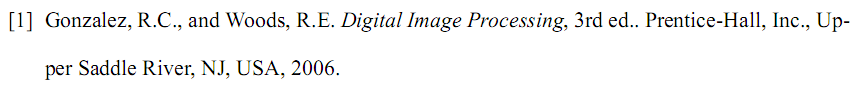
\includegraphics[width=\textwidth]{gonzalez.png}

این شیوه برای تعداد مراجع کم بد نیست اما اگر فرمت مراجع، ترتیب یا تعداد آنها را خواسته باشید تغییر دهید، به عنوان مثال ابتدا حرف اول نام نویسنده بیاید و سپس نام خانوادگی، باید همه کارها را به صورت دستی انجام دهید.
اگر مایلید کنترل کاملی بر مراجع خود داشته باشید و به راحتی بتوانید قالب مراجع خود را عوض کنید باید از \lr{Bib\TeX} استفاده کنید که درپیوست  \ref{App:RefMan} به  آن پرداخته خواهد شد.
!
را در فایل 
\lr{main.tex}،
غیرفعال%
\footnote{
برای غیرفعال کردن یک دستور، کافی است در ابتدای آن، یک علامت
\%
 بگذارید.
}
 کنید.  در غیر این صورت، ابتدا مطالب دو فصل اول  پردازش شده و سپس مطالب فصل ۳ پردازش می‌شود و این کار باعث طولانی شدن زمان اجرا می‌شود. هر زمان که خروجی کل \پ خود را خواستید تمام فصلها را از حالت توضیح خارج کنید.

\subsection{مراجع}
برای وارد کردن مراجع \پ خود، کافی است فایل 
\lr{MyReferences.bib}
را باز کرده و مراجع خود را مانند مراجع داخل آن، وارد کنید.  سپس از \lr{bibtex} برای تولید مراجع با قالب مناسب استفاده کنید. برای توضیحات بیشتر بخش \ref{Sec:Ref} و پیوست \ref{App:RefMan} را ببینید.


\subsection{واژه‌نامه فارسی به انگلیسی و برعکس}
برای وارد کردن واژه‌نامه فارسی به انگلیسی و برعکس، چنانچه کاربر مبتدی هستید، بهتر است مانند روش بکار رفته در فایل‌های 
\lr{dicfa2en}
و
\lr{dicen2fa}
عمل کنید. اما چنانچه کاربر پیشرفته هستید، بهتر است از بسته
\lr{glossaries}
استفاده کنید. راهنمای این بسته را می‌توانید به راحتی و با یک جستجوی ساده در اینترنت پیدا کنید.
\subsection{نمایه}
برای وارد کردن نمایه، باید از 
\lr{xindy}
استفاده کنید. 
%زیرا 
%\lr{MakeIndex}
%با حروف «گ»، «چ»، «پ»، «ژ» و «ک» مشکل دارد و ترتیب الفبایی این حروف را رعایت نمی‌کند. همچنین، فاصله بین هر گروه از کلمات در 
%\lr{MakeIndex}،
%به درستی رعایت نمی‌شود که باعث زشت شدن حروف‌چینی این قسمت می‌شود. 
راهنمای چگونگی کار با 
\lr{xindy} 
را می‌توانید در تالار گفتگوی پارسی‌لاتک و یا مثالهای موجود در مجموعه پارسی‌لاتک، پیدا کنید.

\section{اگر سوالی داشتم، از کی بپرسم؟}
برای پرسیدن سوال‌های خود موقع حروف‌چینی با زی‌پرشین،  می‌توانید به
 \href{http://forum.parsilatex.com}{تالار گفتگوی پارسی‌لاتک}%
\LTRfootnote{http://forum.parsilatex.com}
مراجعه کنید. شما هم می‌توانید روزی به سوال‌های دیگران در این تالار، جواب بدهید.
    
\section{جمع‌بندی}
بسته‌ی زی‌پرشین و بسیاری بسته‌های مرتبط با آن مانند \lr{bidi} و \lr{Persian-bib}، مجموعه پارسی‌لاتک، مثالهای مختلف موجود در آن، استیلهای مختلف پایان‌نامه دانشگاههای مختلف، سایت پارسی‌لاتک همه به صورت داوطلبانه توسط افراد گروه پارسی‌لاتک و بدون هیچ کمک مالی انجام شده‌اند. کار اصلی نوشتن و توسعه زی‌پرشین توسط آقای وفا خلیقی انجام شده است که این کار بزرگ را به انجام رساندند.
اگر مایل به کمک مالی به گروه پارسی‌لاتک هستید کمک‌های مالی خود را به  شماره حساب 
زیر نزد بانک ملی، به نام هادی صفی‌اقدم واریز نمایید:
\begin{center}
شماره حساب: ۰۱۰۱۲۰۰۰۷۰۰۰۳

شماره کارت: 
\lr{6037-9910-4168-7363}

شماره شبا: 
\lr{IR72-0170-0000-0010-1200-0700-03}
\end{center}
لطفاً پس از واریز وجه، موضوع را از طریق ایمیل به آقای صفی‌اقدم اطلاع دهید (\lr{hadi.safiaghdam@gmail.com}).!
و
\verb!% !TeX root=main.tex
\chapter{آشنایی سریع با برخی دستورات لاتک}\label{Chap:latexIntro}
\thispagestyle{empty}
در این فصل ویژگی‌های مهم و پرکاربرد زی‌پرشین و لاتک معرفی می‌شود. برای راهنمایی بیشتر و به‌کاربردن ویژگی‌های پیشرفته‌تر به راهنمای زی‌پرشین و راهنمای لاتک مراجعه کنید. برای آگاهی از دستورات لاتک که این خروجی را تولید کرده‌اند فایل \lr{latexIntro.tex} را ملاحظه فرمایید.
\footnote{بیشتر مطالب این بخش از مثال 
\lr{xepersian\_example.tex}
گرفته شده‌اند که توسط دوستمان آقای امیرمسعود پورموسی آماده شده بوده است.}

\section{بندها و زیرنویس‌ها}
هر جایی از نوشتهٔ خود، اگر می‌خواهید به سر سطر بروید و یک بند تازه را آغاز کنید، باید یک خط را خالی بگذارید
\footnote{یعنی دوبار باید کلید \lr{Enter} را بزنید.}
 مانند این:

حالا که یک بند تازه آغاز شده است، یک زیرنویس انگلیسی
\LTRfootnote{English Footnote!}
 هم می‌نویسیم!
\section{فرمول‌های ریاضی}\label{formula}

اینجا هم یک فرمول می‌آوریم که شماره دارد:
\begin{equation}\label{eq:yek}
A=\frac{c}{d}+\frac{q^2}{\sin(\omega t)+\Omega_{12}}
\end{equation}
در لاتک می‌توان به کمک فرمان 
\lr{\textbackslash label\{\}}
به هر فرمول یک نام نسبت داد. در فرمول بالا نام \lr{eq:yek} را برایش گذاشته‌ایم (پروندهٔ \lr{tex} همراه با این مثال را ببینید). این نام ما را قادر می‌کند که بعداً بتوانیم با فرمان
\lr{\textbackslash ref\{eq:yek\}}
به آن فرمول با شماره ارجاع دهیم. یعنی بنویسیم فرمول \ref{eq:yek}. 
لاتک خودش شمارهٔ این فرمول‌ها را مدیریت می‌کند.\footnote{یعنی اگر بعداً فرمولی قبل از این فرمول بنویسیم، خودبه‌خود شمارهٔ این فرمول و شمارهٔ ارجاع‌ها به این فرمول یکی زیاد می‌شود. دیگر نگران شماره‌گذاری فرمول‌های خود نباشید!} این هم یک فرمول که شماره ندارد:
$$A=|\vec{a}\times \vec{b}| + \sum_{n=0}^\infty C_{ij}$$

این هم عبارتی ریاضی مانند 
$\sqrt{a^2+b^2}$
 که بین متن می‌آید.
\subsection{یک زیربخش}\label{zirbakhsh}

این زیربخش \ref{zirbakhsh} است؛ یعنی یک بخش درون بخش \ref{formula} است.
\subsubsection{یک زیرزیربخش}
این هم یک زیرزیربخش است. در لاتک می‌توانید بخش‌های تودرتو در نوشته‌تان تعریف کنید تا ساختار منطقی نوشته را به خوبی نشان دهید. می‌توانید به این بخش‌ها هم با شماره ارجاع دهید، مثلاً بخش فرمول‌های ریاضی شماره‌اش \ref{formula} است.
\section{نوشته‌های فارسی و انگلیسی مخلوط}
نوشتن یک کلمهٔ انگلیسی بین متن فارسی بدیهی است، مانند Example در این جمله.
نوشتن یک عبارت چندکلمه‌ای مانند
 \lr{More than one word} کمی پیچیده‌تر است.

اگر ناگهان تصمیم بگیرید که یک بند کاملاً انگلیسی را بنویسید، باید:
\begin{latin}
This is an English paragraph from left to right. You can write as much as you want in it.
\end{latin}
\section{افزودن تصویر به نوشته}
پروندهٔ تصویر دلخواه خود را در کنار پروندهٔ \lr{tex} قرار دهید. سپس به روش زیر تصویر را در نوشتهٔ خود بیاورید:
\begin{latin}
\begin{verbatim}
\includegraphics{YourImageFileName}
\end{verbatim}
\end{latin}
به تصویرها هم مانند فرمول‌ها و بخش‌ها می‌توان با شماره ارجاع داد. مثلاً تصویر  \ref{fig:shir} یک شیر علاقه‌مند به لاتک را در حال دویدن نشان می‌دهد. برای جزئیات بیشتر دربارهٔ روش گذاشتن تصویرها در نوشته باید راهنماهای لاتک را بخوانید.
\begin{figure}%[ht]
\centerline{
\includegraphics[width=5cm]{lion}}
\caption{در این تصویر یک شیر علاقه‌مند به لاتک را در حال دویدن می‌بینید.}
\label{fig:shir}
\end{figure}

به تصویرها هم مانند فرمول‌ها و بخش‌ها می‌توان با شماره ارجاع داد. مثلاً تصویر بالا شماره‌اش \ref{fig:shir} است. برای جزئیات بیشتر دربارهٔ روش گذاشتن تصویرها در نوشته باید راهنماهای لاتک را بخوانید.

\section{محیط‌های شمارش و نکات}
برای فهرست‌کردن چندمورد، اگر ترتیب برایمان مهم نباشد:
\begin{itemize}
\item مورد یکم
\item مورد دوم
\item مورد سوم
\end{itemize}
و اگر ترتیب برایمان مهم باشد:
\begin{enumerate}
\item مورد یکم
\item مورد دوم
\item مورد سوم
\end{enumerate}
می‌توان موردهای تودرتو داشت:
\begin{enumerate}
\item مورد ۱
\item مورد ۲
\begin{enumerate}
\item مورد ۱ از ۲
\item مورد ۲ از ۲
\item مورد ۳ از ۲
\end{enumerate}
\item مورد ۳
\end{enumerate}
شماره‌گذاری این موردها را هم لاتک انجام می‌دهد.

\section{تعریف و قضیه}
برای ذکر تعریف، قضیه و مثال مثالهای ذیل را ببینید.
\begin{definition}
مجموعه همه ارزیابی‌های  (پیوسته)  روی $(X,\tau)$، دامنه توانی احتمالی
\index{دامنه توانی احتمالی}
$ X $
نامیده می‌شود.
\end{definition}
\begin{theorem}[باناخ-آلااغلو]
\index{قضیه باناخ-آلااغلو}
اگر $ V $ یک همسایگی $ 0 $ در فضای برداری 
\index{فضای!برداری}
 توپولوژیکی $ X $ باشد و 
\begin{equation}\label{eq1}
K=\left\lbrace \Lambda \in X^{*}:|\Lambda x|\leqslant 1 ; \ \forall x\in V\right\rbrace,
\end{equation}
آنگاه $ K $،  ضعیف*-فشرده است که در آن، $ X^{*} $ دوگان
\index{فضای!دوگان}
 فضای برداری توپولوژیکی $ X $ است به ‌طوری که عناصر آن،  تابعی‌های 
خطی پیوسته
\index{تابعی خطی پیوسته}
 روی $X$ هستند.
\end{theorem}
تساوی \eqref{eq1} یکی از مهم‌ترین تساوی‌ها در آنالیز تابعی است که در ادامه، به وفور از آن استفاده می‌شود.
\begin{example}
برای هر فضای مرتب، گردایه 
$$U:=\left\lbrace U\in O: U=\uparrow U\right\rbrace $$
از مجموعه‌های بالایی باز، یک توپولوژی تعریف می‌کند که از توپولوژی اصلی، درشت‌تر  است.
\end{example}
حال تساوی 
\begin{equation}\label{eq2}
\sum_{n=1}^{+\infty} 3^{n}x+7x=\int_{1}^{n}8nx+\exp{(2nx)}
\end{equation}
را در نظر بگیرید. با مقایسه تساوی \eqref{eq2} با تساوی \eqref{eq1} می‌توان نتیجه گرفت که ...


\section{چگونگی نوشتن و ارجاع به مراجع}\label{Sec:Ref}

در لاتک به راحتی می‌توان مراجع خود را نوشت و به آنها ارجاع داد. به عنوان مثال برای معرفی کتاب گنزالس \cite{Gonzalez02book} به عنوان یک مرجع می‌توان آنرا به صورت زیر معرفی نمود:

\singlespacing
\begin{LTR}
\begin{verbatim}
\bibitem{Gonzalez02book}
Gonzalez, R.C., and Woods, R.E. {\em Digital Image Processing}, 3rd ed..
Prentice-Hall, Inc., Upper Saddle River, NJ, USA, 2006.
\end{verbatim}
\end{LTR}
\doublespacing

در دستورات فوق \lr{Gonzalez02book}  برچسبی است که به این مرجع داده شده است و با استفاده از دستور 
\verb!\cite{Gonzalez02book}!
می‌توان به آن ارجاع داد؛ بدون این که شماره‌اش را در فهرست مراجع‌مان بدانیم.

اگر این اولین مرجع ما باشد در قسمت مراجع به صورت زیر خواهد آمد:\\
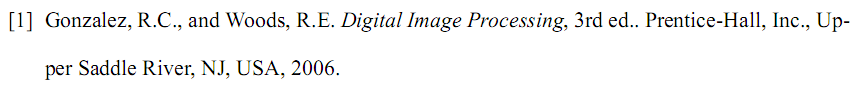
\includegraphics[width=\textwidth]{gonzalez.png}

این شیوه برای تعداد مراجع کم بد نیست اما اگر فرمت مراجع، ترتیب یا تعداد آنها را خواسته باشید تغییر دهید، به عنوان مثال ابتدا حرف اول نام نویسنده بیاید و سپس نام خانوادگی، باید همه کارها را به صورت دستی انجام دهید.
اگر مایلید کنترل کاملی بر مراجع خود داشته باشید و به راحتی بتوانید قالب مراجع خود را عوض کنید باید از \lr{Bib\TeX} استفاده کنید که درپیوست  \ref{App:RefMan} به  آن پرداخته خواهد شد.
!
را در فایل 
\lr{main.tex}،
غیرفعال%
\footnote{
برای غیرفعال کردن یک دستور، کافی است در ابتدای آن، یک علامت
\%
 بگذارید.
}
 کنید.  در غیر این صورت، ابتدا مطالب دو فصل اول  پردازش شده و سپس مطالب فصل ۳ پردازش می‌شود و این کار باعث طولانی شدن زمان اجرا می‌شود. هر زمان که خروجی کل \پ خود را خواستید تمام فصلها را از حالت توضیح خارج کنید.

\subsection{مراجع}
برای وارد کردن مراجع \پ خود، کافی است فایل 
\lr{MyReferences.bib}
را باز کرده و مراجع خود را مانند مراجع داخل آن، وارد کنید.  سپس از \lr{bibtex} برای تولید مراجع با قالب مناسب استفاده کنید. برای توضیحات بیشتر بخش \ref{Sec:Ref} و پیوست \ref{App:RefMan} را ببینید.


\subsection{واژه‌نامه فارسی به انگلیسی و برعکس}
برای وارد کردن واژه‌نامه فارسی به انگلیسی و برعکس، چنانچه کاربر مبتدی هستید، بهتر است مانند روش بکار رفته در فایل‌های 
\lr{dicfa2en}
و
\lr{dicen2fa}
عمل کنید. اما چنانچه کاربر پیشرفته هستید، بهتر است از بسته
\lr{glossaries}
استفاده کنید. راهنمای این بسته را می‌توانید به راحتی و با یک جستجوی ساده در اینترنت پیدا کنید.
\subsection{نمایه}
برای وارد کردن نمایه، باید از 
\lr{xindy}
استفاده کنید. 
%زیرا 
%\lr{MakeIndex}
%با حروف «گ»، «چ»، «پ»، «ژ» و «ک» مشکل دارد و ترتیب الفبایی این حروف را رعایت نمی‌کند. همچنین، فاصله بین هر گروه از کلمات در 
%\lr{MakeIndex}،
%به درستی رعایت نمی‌شود که باعث زشت شدن حروف‌چینی این قسمت می‌شود. 
راهنمای چگونگی کار با 
\lr{xindy} 
را می‌توانید در تالار گفتگوی پارسی‌لاتک و یا مثالهای موجود در مجموعه پارسی‌لاتک، پیدا کنید.

\section{اگر سوالی داشتم، از کی بپرسم؟}
برای پرسیدن سوال‌های خود موقع حروف‌چینی با زی‌پرشین،  می‌توانید به
 \href{http://forum.parsilatex.com}{تالار گفتگوی پارسی‌لاتک}%
\LTRfootnote{http://forum.parsilatex.com}
مراجعه کنید. شما هم می‌توانید روزی به سوال‌های دیگران در این تالار، جواب بدهید.
    
\section{جمع‌بندی}
بسته‌ی زی‌پرشین و بسیاری بسته‌های مرتبط با آن مانند \lr{bidi} و \lr{Persian-bib}، مجموعه پارسی‌لاتک، مثالهای مختلف موجود در آن، استیلهای مختلف پایان‌نامه دانشگاههای مختلف، سایت پارسی‌لاتک همه به صورت داوطلبانه توسط افراد گروه پارسی‌لاتک و بدون هیچ کمک مالی انجام شده‌اند. کار اصلی نوشتن و توسعه زی‌پرشین توسط آقای وفا خلیقی انجام شده است که این کار بزرگ را به انجام رساندند.
اگر مایل به کمک مالی به گروه پارسی‌لاتک هستید کمک‌های مالی خود را به  شماره حساب 
زیر نزد بانک ملی، به نام هادی صفی‌اقدم واریز نمایید:
\begin{center}
شماره حساب: ۰۱۰۱۲۰۰۰۷۰۰۰۳

شماره کارت: 
\lr{6037-9910-4168-7363}

شماره شبا: 
\lr{IR72-0170-0000-0010-1200-0700-03}
\end{center}
لطفاً پس از واریز وجه، موضوع را از طریق ایمیل به آقای صفی‌اقدم اطلاع دهید (\lr{hadi.safiaghdam@gmail.com}).!
و
\verb!% !TeX root=main.tex
\chapter{آشنایی سریع با برخی دستورات لاتک}\label{Chap:latexIntro}
\thispagestyle{empty}
در این فصل ویژگی‌های مهم و پرکاربرد زی‌پرشین و لاتک معرفی می‌شود. برای راهنمایی بیشتر و به‌کاربردن ویژگی‌های پیشرفته‌تر به راهنمای زی‌پرشین و راهنمای لاتک مراجعه کنید. برای آگاهی از دستورات لاتک که این خروجی را تولید کرده‌اند فایل \lr{latexIntro.tex} را ملاحظه فرمایید.
\footnote{بیشتر مطالب این بخش از مثال 
\lr{xepersian\_example.tex}
گرفته شده‌اند که توسط دوستمان آقای امیرمسعود پورموسی آماده شده بوده است.}

\section{بندها و زیرنویس‌ها}
هر جایی از نوشتهٔ خود، اگر می‌خواهید به سر سطر بروید و یک بند تازه را آغاز کنید، باید یک خط را خالی بگذارید
\footnote{یعنی دوبار باید کلید \lr{Enter} را بزنید.}
 مانند این:

حالا که یک بند تازه آغاز شده است، یک زیرنویس انگلیسی
\LTRfootnote{English Footnote!}
 هم می‌نویسیم!
\section{فرمول‌های ریاضی}\label{formula}

اینجا هم یک فرمول می‌آوریم که شماره دارد:
\begin{equation}\label{eq:yek}
A=\frac{c}{d}+\frac{q^2}{\sin(\omega t)+\Omega_{12}}
\end{equation}
در لاتک می‌توان به کمک فرمان 
\lr{\textbackslash label\{\}}
به هر فرمول یک نام نسبت داد. در فرمول بالا نام \lr{eq:yek} را برایش گذاشته‌ایم (پروندهٔ \lr{tex} همراه با این مثال را ببینید). این نام ما را قادر می‌کند که بعداً بتوانیم با فرمان
\lr{\textbackslash ref\{eq:yek\}}
به آن فرمول با شماره ارجاع دهیم. یعنی بنویسیم فرمول \ref{eq:yek}. 
لاتک خودش شمارهٔ این فرمول‌ها را مدیریت می‌کند.\footnote{یعنی اگر بعداً فرمولی قبل از این فرمول بنویسیم، خودبه‌خود شمارهٔ این فرمول و شمارهٔ ارجاع‌ها به این فرمول یکی زیاد می‌شود. دیگر نگران شماره‌گذاری فرمول‌های خود نباشید!} این هم یک فرمول که شماره ندارد:
$$A=|\vec{a}\times \vec{b}| + \sum_{n=0}^\infty C_{ij}$$

این هم عبارتی ریاضی مانند 
$\sqrt{a^2+b^2}$
 که بین متن می‌آید.
\subsection{یک زیربخش}\label{zirbakhsh}

این زیربخش \ref{zirbakhsh} است؛ یعنی یک بخش درون بخش \ref{formula} است.
\subsubsection{یک زیرزیربخش}
این هم یک زیرزیربخش است. در لاتک می‌توانید بخش‌های تودرتو در نوشته‌تان تعریف کنید تا ساختار منطقی نوشته را به خوبی نشان دهید. می‌توانید به این بخش‌ها هم با شماره ارجاع دهید، مثلاً بخش فرمول‌های ریاضی شماره‌اش \ref{formula} است.
\section{نوشته‌های فارسی و انگلیسی مخلوط}
نوشتن یک کلمهٔ انگلیسی بین متن فارسی بدیهی است، مانند Example در این جمله.
نوشتن یک عبارت چندکلمه‌ای مانند
 \lr{More than one word} کمی پیچیده‌تر است.

اگر ناگهان تصمیم بگیرید که یک بند کاملاً انگلیسی را بنویسید، باید:
\begin{latin}
This is an English paragraph from left to right. You can write as much as you want in it.
\end{latin}
\section{افزودن تصویر به نوشته}
پروندهٔ تصویر دلخواه خود را در کنار پروندهٔ \lr{tex} قرار دهید. سپس به روش زیر تصویر را در نوشتهٔ خود بیاورید:
\begin{latin}
\begin{verbatim}
\includegraphics{YourImageFileName}
\end{verbatim}
\end{latin}
به تصویرها هم مانند فرمول‌ها و بخش‌ها می‌توان با شماره ارجاع داد. مثلاً تصویر  \ref{fig:shir} یک شیر علاقه‌مند به لاتک را در حال دویدن نشان می‌دهد. برای جزئیات بیشتر دربارهٔ روش گذاشتن تصویرها در نوشته باید راهنماهای لاتک را بخوانید.
\begin{figure}%[ht]
\centerline{
\includegraphics[width=5cm]{lion}}
\caption{در این تصویر یک شیر علاقه‌مند به لاتک را در حال دویدن می‌بینید.}
\label{fig:shir}
\end{figure}

به تصویرها هم مانند فرمول‌ها و بخش‌ها می‌توان با شماره ارجاع داد. مثلاً تصویر بالا شماره‌اش \ref{fig:shir} است. برای جزئیات بیشتر دربارهٔ روش گذاشتن تصویرها در نوشته باید راهنماهای لاتک را بخوانید.

\section{محیط‌های شمارش و نکات}
برای فهرست‌کردن چندمورد، اگر ترتیب برایمان مهم نباشد:
\begin{itemize}
\item مورد یکم
\item مورد دوم
\item مورد سوم
\end{itemize}
و اگر ترتیب برایمان مهم باشد:
\begin{enumerate}
\item مورد یکم
\item مورد دوم
\item مورد سوم
\end{enumerate}
می‌توان موردهای تودرتو داشت:
\begin{enumerate}
\item مورد ۱
\item مورد ۲
\begin{enumerate}
\item مورد ۱ از ۲
\item مورد ۲ از ۲
\item مورد ۳ از ۲
\end{enumerate}
\item مورد ۳
\end{enumerate}
شماره‌گذاری این موردها را هم لاتک انجام می‌دهد.

\section{تعریف و قضیه}
برای ذکر تعریف، قضیه و مثال مثالهای ذیل را ببینید.
\begin{definition}
مجموعه همه ارزیابی‌های  (پیوسته)  روی $(X,\tau)$، دامنه توانی احتمالی
\index{دامنه توانی احتمالی}
$ X $
نامیده می‌شود.
\end{definition}
\begin{theorem}[باناخ-آلااغلو]
\index{قضیه باناخ-آلااغلو}
اگر $ V $ یک همسایگی $ 0 $ در فضای برداری 
\index{فضای!برداری}
 توپولوژیکی $ X $ باشد و 
\begin{equation}\label{eq1}
K=\left\lbrace \Lambda \in X^{*}:|\Lambda x|\leqslant 1 ; \ \forall x\in V\right\rbrace,
\end{equation}
آنگاه $ K $،  ضعیف*-فشرده است که در آن، $ X^{*} $ دوگان
\index{فضای!دوگان}
 فضای برداری توپولوژیکی $ X $ است به ‌طوری که عناصر آن،  تابعی‌های 
خطی پیوسته
\index{تابعی خطی پیوسته}
 روی $X$ هستند.
\end{theorem}
تساوی \eqref{eq1} یکی از مهم‌ترین تساوی‌ها در آنالیز تابعی است که در ادامه، به وفور از آن استفاده می‌شود.
\begin{example}
برای هر فضای مرتب، گردایه 
$$U:=\left\lbrace U\in O: U=\uparrow U\right\rbrace $$
از مجموعه‌های بالایی باز، یک توپولوژی تعریف می‌کند که از توپولوژی اصلی، درشت‌تر  است.
\end{example}
حال تساوی 
\begin{equation}\label{eq2}
\sum_{n=1}^{+\infty} 3^{n}x+7x=\int_{1}^{n}8nx+\exp{(2nx)}
\end{equation}
را در نظر بگیرید. با مقایسه تساوی \eqref{eq2} با تساوی \eqref{eq1} می‌توان نتیجه گرفت که ...


\section{چگونگی نوشتن و ارجاع به مراجع}\label{Sec:Ref}

در لاتک به راحتی می‌توان مراجع خود را نوشت و به آنها ارجاع داد. به عنوان مثال برای معرفی کتاب گنزالس \cite{Gonzalez02book} به عنوان یک مرجع می‌توان آنرا به صورت زیر معرفی نمود:

\singlespacing
\begin{LTR}
\begin{verbatim}
\bibitem{Gonzalez02book}
Gonzalez, R.C., and Woods, R.E. {\em Digital Image Processing}, 3rd ed..
Prentice-Hall, Inc., Upper Saddle River, NJ, USA, 2006.
\end{verbatim}
\end{LTR}
\doublespacing

در دستورات فوق \lr{Gonzalez02book}  برچسبی است که به این مرجع داده شده است و با استفاده از دستور 
\verb!\cite{Gonzalez02book}!
می‌توان به آن ارجاع داد؛ بدون این که شماره‌اش را در فهرست مراجع‌مان بدانیم.

اگر این اولین مرجع ما باشد در قسمت مراجع به صورت زیر خواهد آمد:\\
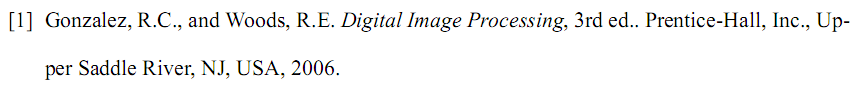
\includegraphics[width=\textwidth]{gonzalez.png}

این شیوه برای تعداد مراجع کم بد نیست اما اگر فرمت مراجع، ترتیب یا تعداد آنها را خواسته باشید تغییر دهید، به عنوان مثال ابتدا حرف اول نام نویسنده بیاید و سپس نام خانوادگی، باید همه کارها را به صورت دستی انجام دهید.
اگر مایلید کنترل کاملی بر مراجع خود داشته باشید و به راحتی بتوانید قالب مراجع خود را عوض کنید باید از \lr{Bib\TeX} استفاده کنید که درپیوست  \ref{App:RefMan} به  آن پرداخته خواهد شد.
!
را در فایل 
\lr{main.tex}،
غیرفعال%
\footnote{
برای غیرفعال کردن یک دستور، کافی است در ابتدای آن، یک علامت
\%
 بگذارید.
}
 کنید.  در غیر این صورت، ابتدا مطالب دو فصل اول  پردازش شده و سپس مطالب فصل ۳ پردازش می‌شود و این کار باعث طولانی شدن زمان اجرا می‌شود. هر زمان که خروجی کل \پ خود را خواستید تمام فصلها را از حالت توضیح خارج کنید.

\subsection{مراجع}
برای وارد کردن مراجع \پ خود، کافی است فایل 
\lr{MyReferences.bib}
را باز کرده و مراجع خود را مانند مراجع داخل آن، وارد کنید.  سپس از \lr{bibtex} برای تولید مراجع با قالب مناسب استفاده کنید. برای توضیحات بیشتر بخش \ref{Sec:Ref} و پیوست \ref{App:RefMan} را ببینید.


\subsection{واژه‌نامه فارسی به انگلیسی و برعکس}
برای وارد کردن واژه‌نامه فارسی به انگلیسی و برعکس، چنانچه کاربر مبتدی هستید، بهتر است مانند روش بکار رفته در فایل‌های 
\lr{dicfa2en}
و
\lr{dicen2fa}
عمل کنید. اما چنانچه کاربر پیشرفته هستید، بهتر است از بسته
\lr{glossaries}
استفاده کنید. راهنمای این بسته را می‌توانید به راحتی و با یک جستجوی ساده در اینترنت پیدا کنید.
\subsection{نمایه}
برای وارد کردن نمایه، باید از 
\lr{xindy}
استفاده کنید. 
%زیرا 
%\lr{MakeIndex}
%با حروف «گ»، «چ»، «پ»، «ژ» و «ک» مشکل دارد و ترتیب الفبایی این حروف را رعایت نمی‌کند. همچنین، فاصله بین هر گروه از کلمات در 
%\lr{MakeIndex}،
%به درستی رعایت نمی‌شود که باعث زشت شدن حروف‌چینی این قسمت می‌شود. 
راهنمای چگونگی کار با 
\lr{xindy} 
را می‌توانید در تالار گفتگوی پارسی‌لاتک و یا مثالهای موجود در مجموعه پارسی‌لاتک، پیدا کنید.

\section{اگر سوالی داشتم، از کی بپرسم؟}
برای پرسیدن سوال‌های خود موقع حروف‌چینی با زی‌پرشین،  می‌توانید به
 \href{http://forum.parsilatex.com}{تالار گفتگوی پارسی‌لاتک}%
\LTRfootnote{http://forum.parsilatex.com}
مراجعه کنید. شما هم می‌توانید روزی به سوال‌های دیگران در این تالار، جواب بدهید.
    
\section{جمع‌بندی}
بسته‌ی زی‌پرشین و بسیاری بسته‌های مرتبط با آن مانند \lr{bidi} و \lr{Persian-bib}، مجموعه پارسی‌لاتک، مثالهای مختلف موجود در آن، استیلهای مختلف پایان‌نامه دانشگاههای مختلف، سایت پارسی‌لاتک همه به صورت داوطلبانه توسط افراد گروه پارسی‌لاتک و بدون هیچ کمک مالی انجام شده‌اند. کار اصلی نوشتن و توسعه زی‌پرشین توسط آقای وفا خلیقی انجام شده است که این کار بزرگ را به انجام رساندند.
اگر مایل به کمک مالی به گروه پارسی‌لاتک هستید کمک‌های مالی خود را به  شماره حساب 
زیر نزد بانک ملی، به نام هادی صفی‌اقدم واریز نمایید:
\begin{center}
شماره حساب: ۰۱۰۱۲۰۰۰۷۰۰۰۳

شماره کارت: 
\lr{6037-9910-4168-7363}

شماره شبا: 
\lr{IR72-0170-0000-0010-1200-0700-03}
\end{center}
لطفاً پس از واریز وجه، موضوع را از طریق ایمیل به آقای صفی‌اقدم اطلاع دهید (\lr{hadi.safiaghdam@gmail.com}).